\documentclass[12pt, a4paper]{memoir} % for a short document
\usepackage[french,english]{babel}

\usepackage [vscale=0.76,includehead]{geometry}                % See geometry.pdf to learn the layout options. There are lots.
%\geometry{a4paper}                   % ... or a4paper or a5paper or ...
%\geometry{landscape}                % Activate for for rotated page geometry
%\OnehalfSpacing
% \setSingleSpace{1.05}
%\usepackage[parfill]{parskip}    % Activate to begin paragraphs with an empty line rather than an indent
\usepackage{graphicx}
\usepackage{amsmath}
\usepackage{fullpage}
\usepackage{mathptmx} % font = times
\usepackage{helvet} % font sf = helvetica
\usepackage[latin1]{inputenc}
\usepackage{relsize}
\usepackage{listings}
\usepackage{gensymb}
\usepackage{hyperref}
\usepackage[usenames,dvipsnames,svgnames,table]{xcolor}

\lstset{
	basicstyle=\footnotesize,
	numbers=left,
	numbersep=7pt,
	escapeinside={<@}{@>}
}

%Style des têtes de section, headings, chapitre
\headstyles{komalike}
\nouppercaseheads
\chapterstyle{dash}
\makeevenhead{headings}{\sffamily\thepage}{}{\sffamily\leftmark}
\makeoddhead{headings}{\sffamily\rightmark}{}{\sffamily\thepage}
\makeoddfoot{plain}{}{}{} % Pages chapitre.
\makeheadrule{headings}{\textwidth}{\normalrulethickness}
%\renewcommand{\leftmark}{\thechapter ---}
\renewcommand{\chaptername}{\relax}
\renewcommand{\chaptitlefont}{ \sffamily\bfseries \LARGE}
\renewcommand{\chapnumfont}{ \sffamily\bfseries \LARGE}
\setsecnumdepth{subsection}

\newcommand{\eg}{\emph{e.g.~}}
\newcommand{\ie}{\emph{i.e.~}}

% Title page formatting -- do not change!
\pretitle{\HUGE\sffamily \bfseries\begin{center}}
\posttitle{\end{center}}
\preauthor{\LARGE  \sffamily \bfseries\begin{center}}
\postauthor{\par\end{center}}

\newcommand{\jury}[1]{%
\gdef\juryB{#1}}
\newcommand{\juryB}{}
\newcommand{\session}[1]{%
\gdef\sessionB{#1}}
\newcommand{\sessionB}{}
\newcommand{\option}[1]{%
\gdef\optionB{#1}}
\newcommand{\optionB}{}

\renewcommand{\maketitlehookd}{%
\vfill{}  \large\par\noindent
\begin{center}\juryB \bigskip\sessionB\end{center}
\vspace{-1.5cm}}
\renewcommand{\maketitlehooka}{%
\vspace{-1.5cm}\noindent
\includegraphics[height=14ex]{logoINP.png}\hfill\raisebox{2ex}{
\includegraphics[height=7ex]{logoUJF.jpg}}\\
\bigskip
\begin{center} \large
Master of Science in Informatics at Grenoble \\
Master Math\'ematiques Informatique - sp\'ecialit\'e Informatique \\
option \optionB  \end{center}\vfill}
% End of title page formatting

\option{Artificial Intelligence and the Web}
\title{BDI multi-agent modelling of the population's decision making in a bushfire}%\\\vspace{-1ex}\rule{10ex}{0.5pt} \\sub-title}
\author{Geoffrey Danet}
\date{June 22, 2016} % Delete this line to display the current date
\jury{
Research project performed at Laboratoire d'Informatique de Grenoble (LIG) \\\medskip
Under the supervision of:\\
Dr Carole Adam, Laboratoire d'Informatique de Grenoble (LIG)\\\medskip
Defended before a jury composed of:\\
Prof N. Brauner\\
Prof M. Reza Amani\\
Prof C. Berrut\\
Prof J. Euzenat\\
Prof E. Gaussier\\
Dr B. Lemaire\\
}
\session{June\hfill 2016}

%%% BEGIN DOCUMENT
\begin{document}
\selectlanguage{english} % french si rapport en français
\frontmatter
\begin{titlingpage}
\maketitle
\end{titlingpage}

%\small
\setlength{\parskip}{-1pt plus 1pt}

\renewcommand{\abstracttextfont}{\normalfont}
\abstractintoc
\begin{abstract}
	Each summer in Australia, bushfires burn many hectares of forest, causing deaths, injuries, and destruction of property.
	Unfortunately, the emergency services strategy is made according to their own point of view about the citizens' behaviour,
	which does not always match reality. In order to raise their awareness about the real population behaviour, we want to
	provide them with a serious game. The underlying agent-based simulation must be as realistic as possible.
	The philosophically-grounded BDI architecture provides a high level of abstraction and is therefore the most suitable
	approach. We proposes a BDI multi-agent simulation of citizen behaviour during a bushfire, based on the witness statements,
	and validated from statistics.
\end{abstract}

\newpage

\abstractintoc
\renewcommand\abstractname{Acknowledgement}
\begin{abstract}
	Carole Adam,
	Julie Dugdale,
	Benoit Gaudou (GAMA),
	Patrick Taillandier (GAMA),
	Philippe Caillou (GAMA),
	Mathieu Bourgais (GAMA),
	John Thangarajah (TDF),
	Julius Millano Ba\~ngate,
	Antoine Faravelon
\end{abstract}
\selectlanguage{english}% french si rapport en français

\cleardoublepage

\tableofcontents* % the asterisk means that the table of contents itself isn't put into the ToC
\normalsize

\mainmatter
\SingleSpace

\chapter{Introduction}

  On Saturday 7th February 2009, the region of Victoria (Australia) was the victim of violent bushfire causing 173 deaths and many injured.
	The Victoria area endured the most severe and prolonged heatwaves during the final week of January 2009. The temperature was above 43\degree C during three consecutive days.
	The saturday was one of the worse day with in addition to the high temperature (from 40\degree C the morning to 46.4\degree C at the hottest period of the day at Melbourne) a strong wind (around 100 km/h).
	Moreover, the Country Fire Authority (CFA) and the Department of Sustainability and Environment (DSE) warned the citizens that forests and grasslands were the driest they had been since 1983.
	During this day, the extreme conditions triggered 15 fires. The consequence of the fires was the death of 173 peoples, 414 injured, 450,000 hectares (4,500 \begin{math}km^{2}\end{math}) burned.
  Reports showed that there was a discrepancy between how the emergency services expected the population to behave, and how they really behaved \cite{rhodes2014}.
  The problem is that emergency strategies were based on this expected behaviour rather than on the real one.

	\paragraph{}
	\textbf{SWIFT project}
	\paragraph{}

	The focus of this project is to provide a serious game for the emergency managers in order to test various strategies and finally help them to take the best decision.
	For that, the model of the population must be as accurate as possible. The SWIFT project is interested in modelling and simulating the population behaviour in the state of Victoria in Australia during a bushfire.
	The approach is agent-based modelling and simulation, with a BDI (Belief, Desire, Intention) architecture of the agents, to endow them with a
	realistic behaviour based on psychological theories, as well as on field studies and witness statements made by the Victorian Bushfires Royal Commission (VBRC).

	\paragraph{}
	The contributions during this internship were the implementation of a BDI architecture initially based on a finite state machine architecture. We propose as well a
	methodology in order to convert interview data (textual data) in BDI with a low requirement in computer science.

	\paragraph{}
	At first, we will describe the existing studies in simulation for crisis situations. Secondly, we will describe the tools and the methodology used during this project.
	After what, we will describe the data used and the current implementation. To finish, we show some results and make a conclusion.


%=====================
\chapter{State Of the Art}

	Many crisis situations occur in this world, which can cause both psychological and physical injuries besides considerable damages which have an important cost on the economy.
	In order to reduce the impact of such situations, many countries are actively searching ways to prevent crisis and decrease the potential number of victims.
	The observation was the first source of knowledge, but implies victims as well. Quickly, the idea of simulation comes to mind.
	A full-scale simulation is the closest solution to get realistic results but is very costly, impossible to reproduce exactly, and of course can be very dangerous.
	On the other hand, we have the computer simulation which provides a cheap, infinitely reusable, and safe solution but with a less realistic result.
	Moreover, this kind of simulation offers a very high control of the environment and allows to reproduce very precise scenarios easily.
	Computer simulations such as serious game allow subsequently to increase the understanding of more general causal relationship in emergency management
	organizations \cite{ruijven2011}.

	\section{Modelling and Simulation}

		There exist many methods in order to produce simulations.
		Among them, we can find two main categories of simulation models:
		\begin{itemize}
			\item \textbf{Equation-based Model (EBM)}: Model of simulation principally based on differential equation over time.
			A full model can be composed of a succession of equations. Some existing equation used for equation-based simulation
			are famous for this, like for instance the Runge-Kutta method defined by C. Runge and M. W. Kutta in 1990, the Euler method based
			on Leonhard Euler's works (\textit{Institutionum calculi integralis}, 1768) or the Newmark method \cite{newmark1959}.
			This kind of simulation is particulary used in physics for particles simulation \cite{greengard1987} or chemistry for
			molecular dynamics systems\cite{gunsteren1990} for example. %  and epidemiology : des exemples ?
			\item \textbf{Agent-Based Models (ABMs)}: Model of simulation which provide actions and interactions between several
			autonomous entities called agents. Usually, agents are used in a spatiotemporal environment with an automaton architecture
			and can have the possibility to interact with their environment.
		\end{itemize}

		According to a study made by Parunak et al. \cite{parunak1998} the distinction between these two methodologies are essentially in
		the project requirement. ABM is more appropriate for domains with \textquotedblleft \textit{a high degree localization and distribution and dominated by discrete decisions}\textquotedblright.
		EBM is more appropriate for systems where, for exemple, \textquotedblleft \textit{the dynamics are dominated by physical laws rather than information processing.}\textquotedblright.
		Moreover, EBM requires a high knowledge of behaviours and is made for one specific purpose, hence, cannot be easily reused. Thus, a complex system such as cognitive entities
		cannot or is extremely difficult to model using equation in contrary to the ABM modelling systems.

		\subsection{Multi-Agents Systems}

			An agent is a computer system which can interact with its environment in an autonomous way through actions.
			The particularity of multi-agent is the possibility to transfer information between agents. Thanks to the data sharing,
			the agents can, for exemple, collaborate for a task, or ask another agent for information.
			Thanks to that system, an agent which does not have a specific skill to achieve a task, can ask another agent with the
			required skill to do it.
			For exemple, in the context of fire crisis, a citizen can be stuck in a building because of fire (reactive to the environment).
			In order to stay alive, the agent can need to \textbf{inform} firemen about the fire and to \textbf{ask} for help.
			After what, the firemen will extinguish the fire (interaction with the environment).
			The multi-agent simulation provide to the model an easier interaction between their entities.

			The simulation framework of individual cognitive processes attempts to produce emergent social or collaborative behaviour as
			show the study of Pan et al. \cite{pan2007} through a simulation of building evacuations.
			Others studies tried to reproduce the interpretation of risk in the model with a descriptive psychology approach
			during building evacuation.\cite{kinateder2014}.

			\paragraph{}
			% mini conclusion
			Unfortunately, these studies are really specific to the building evacuation domain with consequently a portability problem for other researchers who want to use
			it besides of a higher complexity for the designer.
			Moreover, the low level of abstraction decrease the behaviour comprehension during the simulation. In addition the behaviour trends are the same for all agents.
	    In contrary to these approaches, the BDI (Belief, Desire, Intention) architecture provides a more flexible solution to make an agent simulation.

		\subsection{Belief Desire Intention (BDI)}

			For agents using automatons architecture, the behaviour is defined by the states and its transitions. The agent cannot easily change its intention
			during the simulation if the transitions between these states are not defined. Each transition are determined and defined according to each situation
			and finally result to a similar agent behaviours. To resume, the flexibility of the decision process is dependent upon the automaton implementation.
			In contrast with the automatons, the BDI approaches allows agents to have more realistic behaviours through their own decisions.
			BDI is an agent modelling approaches based on the philosophical theories of Bratman \cite{anand1995}.
			In this architecture, each agent has \textbf{mental states} defined by Belief, Desire and Intention which will affect its behaviour during the simulation.

			\begin{figure}
				\begin{center}
					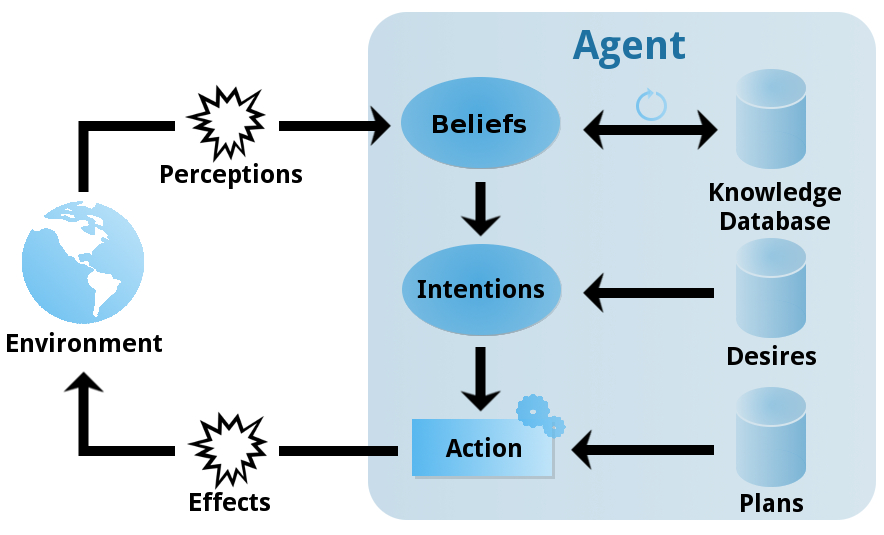
\includegraphics[scale=0.4]{bdi_graph.png}
					\caption{\label{fig:bdi-graph}Basic representation of the BDI architecture.}
				\end{center}
			\end{figure}

			\begin{itemize}
				\item \textbf{Beliefs} represent the agent's informations about the environment, itself or the other agents.
				A belief is not always true, it can be \textbf{incomplete} or \textbf{incorrect}.
				According to these beliefs, the agent can estimate the feasibility of desires and consequently adapt his intentions.
				\newline
				\eg \textquotedblleft I believe that fire will come here soon.\textquotedblright, \textquotedblleft I believe the firemen will deal with it.\textquotedblright.
				\item \textbf{Desires} represent the agent's motivations to do something. Desires have a direct impact on his intentions.
				These desires can be \textbf{inconsistent} or \textbf{unrealistic} and can have differents priorities.
				\newline
				\eg \textquotedblleft I do not want see my house burning.\textquotedblright ~or \textquotedblleft I do not want to be hurt.\textquotedblright
				\item \textbf{Intentions} are selected from the desires and beliefs of the agent. An intention can have several associated plans allowing to achieve it.
				\newline
				\eg The agent believes that fire will come to its place soon, and has the desire to propect its house and to stay alive.
				Consequently, the agent according to its priority will choose between protecting its property if its life is
				not immediately in danger or leaving the house in order to stay alive.
			\end{itemize}

			Obviously, this method fit very well for human behaviour simulation and is more intuitive to use than other approaches.
			Thus, the development of the simulation become easier and more understandable by scientists.

			An example from an extract of witness statement about the Black Saturday :
			\begin{quote}
				\textquotedblleft I looked out the window and saw some hazy smoke to the north-west. Gary said that he thought it was just dust but we went outside and straight away we noticed that we could smell smoke. It was about 12.45pm when we smelt the smoke and as soon as that happened, Gary agreed to go and get the fire pump.\textquotedblright \cite{exell}
			\end{quote}
			This sentence can be easily translated using the BDI architecture, Gary \textbf{believed} for a while that the hazy smoke
			was simply dust but after going outside, they smelt smoke (\textbf{perception}) and realised that the hazy smoke
			was indeed coming from a fire (\textbf{belief update}). Finally, they decide to defend their property (\textbf{intention}),
			with for first \textbf{plan} whose first \textbf{action} is to prepare the fire pump.

			However, BDI does not suit for building systems which must learn and adapt their behaviour and does not have explicitly
			multi-agent aspects of behaviour \cite{georgeff1999}.

			There already exist some BDI framework \cite{caillou2015}:
			\begin{itemize}
				\item Classic framework: Procedural Reasoning System (PRS) which is an architecture for real-time reasoning and system control\cite{ingrand1992}.
				\item Commercial framework: JACK which inherits many properties from PRS and allows to define Multi-Agent Systems (MAS)
				\item The most advanced framework : Jadex, an add-on of the JADE framework which has an explicit representation of goals.
			\end{itemize}

	\section{Egress simulation}

		Egress simulation is a thread which is very studied in crisis simulation and in human behaviors during fire.
		The most studies in egress simulation are focalized on the study of crowds behaviors, dynamics and more precisely on specifics part
		such as risk perception \cite{kinateder2014,mu2013}, communication \cite{pelechano2005}, psychology \cite{pelechano2005,kuligowski2008} and sociology \cite{pan2006,pan2007}.
		Pan et al. \cite{pan2007} categorize the existing model used for crowd in three main categories:
		\begin{itemize}
			\item Fluid of particle systems: used for evacuation simulation, crowds behaviours are similar to fluids.\cite{low2000, helbing2000}
			\item Matrix based systems: The area is represented into cells (grid) where cells represent obstacles, free area, area occuped by a person, ...
			\item Emergent systems: The interactions of simple parts/elements can create an emergeance phenomena and produce complex system (here crowd dynamics)
		\end{itemize}
		Pan et al show that an individual's behaviours follow three basic conventions\cite{pan2006}:
		People how are following instinct, following experience and people who have bounded rationality.
		Another studies about crowd simulation, human behaviours and social behaviours shows several aspect of non-adaptive crowd behaviours.
		Human and social behaviours are categorized in three distinct category: 1) individual (collection of individuals), 2) interactions among individuals and 3) groups. \cite{pan2006}
		% Kuligowski
		Kuligowski introduce a conceptual model of the behavioural process for building fire composed in four phases: 1) Perception of the cue(s), 2) Interpretation of the cue, situation, and risk, 3) decision-making and 4) Actions.
		Unfortunately the level of abstraction is too important to aptly represent the real human behaviours.
		All signals are interpreted in the same way by all agents and does not take in account interpretation such as false warn\cite{kuligowski2008}.

\chapter{Tools and Methodology}

	In this section we introduce the GAMA framework and the Tactical Development Framework used for the modelling and simulation described in this report.

	\section{\label{sec:tdf}Tactics Development Framework}
		Tactics Development Framework (TDF) is a tactical decision-making modelling tool based on the Prometheus methodology \cite{evertsz2015},
		a mature and popular agent-oriented software engineering methodology.
		Made for modern tactical warfare, TDF provides a new way to support the development life cycle of the simulation. The objective
		is to simplify the requirement and knowledge elicitation, then to represent this data through diagrammatic specification.
		Although it was initially made for military tactical purpose, Adam et al. \cite{adam2015} show that TDF suits perfectly for modelling
		the civilian behaviours.

		\subsection{Diagram description}

			This section will introduce the different diagrams provided by TDF. Each diagram is illustrated by an example related to this
			study. The examples and diagrams come from an article which illustrates the methodology used in order to capture civilian's behaviour
			in the fire with TDF and its mapping with GAML code \cite{adam2016}. The model described in these examples is more elaborate than the
			model used during this internship.

			\subsubsection{Analysis overview}

				The goal of this diagram is to identify the different actors (entities external to the system), the inputs (percepts),
				and outputs (actions) and to identify senario (similar to use-cases). In our case,
				the scenarios are exemples of behaviours. A given scenario contains a sequence of steps which include goals (oval shape),
				actions (right arrow), percepts (bang pictogram) and sub-scenarios. The figure~\ref{fig:analysis-overview} shows a part of the
				analysis overview diagram related to a scenario where a Pedestrian defends its property (steps detailed in the figure~\ref{fig:scenario}).

				\begin{figure}
					\begin{center}
						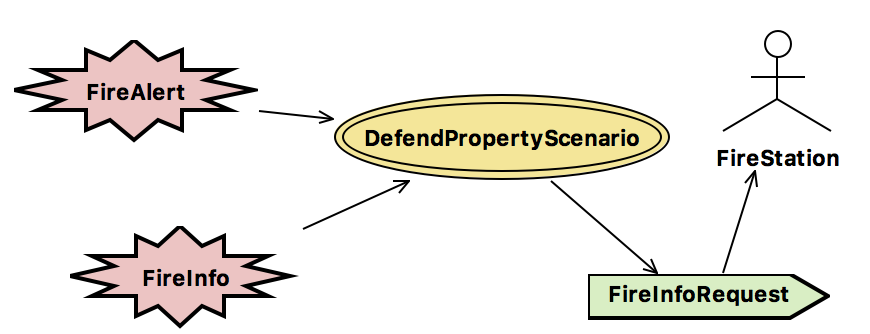
\includegraphics[scale=0.4]{AnalysisOverview.png}
						\caption{\label{fig:analysis-overview}Partial Analysis Overview diagram.}
					\end{center}
				\end{figure}

				\begin{figure}
					\begin{center}
						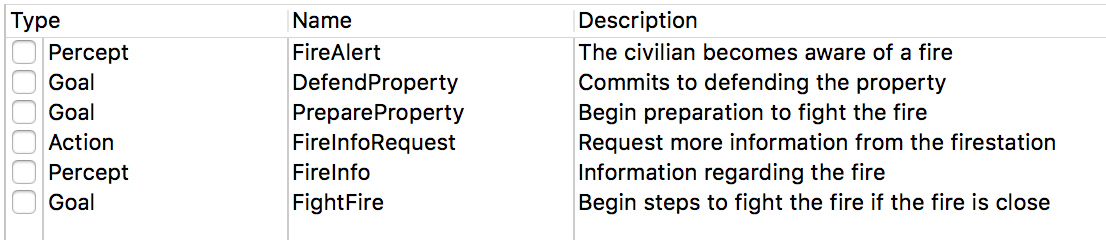
\includegraphics[scale=0.4]{Scenario.png}
						\caption{\label{fig:scenario}Pedestrian defending property (detailed steps).}
					\end{center}
				\end{figure}

			\subsubsection{Goal overview}

				The goal overview diagram illustrates how the high-level goals are decomposed into more concrete goals.
				The figure \ref{fig:goal-overview} represents the goals that Pedestrian can use. These Pedestrians behaviours are
				described in the interviews (see Chapter \ref{chapter:data}) and result from two high-level goals:
				\textbf{Defend property} and \textbf{Stay Alive}. The relative priorities of these goals depend on individual differences
				in various factors: awareness of fire, fire training, motivation to defend property, etc. The sub-goals of a goal can be
				\textit{OR}, \textit{AND} or \textit{CON} decompositions.
				\begin{itemize}
					\item \textit{OR} which correspond to the disjunction: a Pedestrian can try to stay alive by taking cover at home
						\textit{or} by going to a shelter (cannot be both).
					\item \textit{AND} which correspond to the conjunction (can be ordered): to get to a shelter, the Pedestrian agent requires to
						achieve some tasks before: First prepare their house if they are able and if they have enough time to do it (condition), after what
						they must prepare themself, find a shelter spot with a safe road. If the Pedestrian clears these tasks, they can finally go to the
						shelter.
					\item \textit{CON} which mean that sub-goals can be used in parallel. In our example, to fight a fire during the period
						when the fire is far, the Pedestrian can simultaneously prepare their property and seek information about fire status.
				\end{itemize}

				\begin{figure}
					\begin{center}
						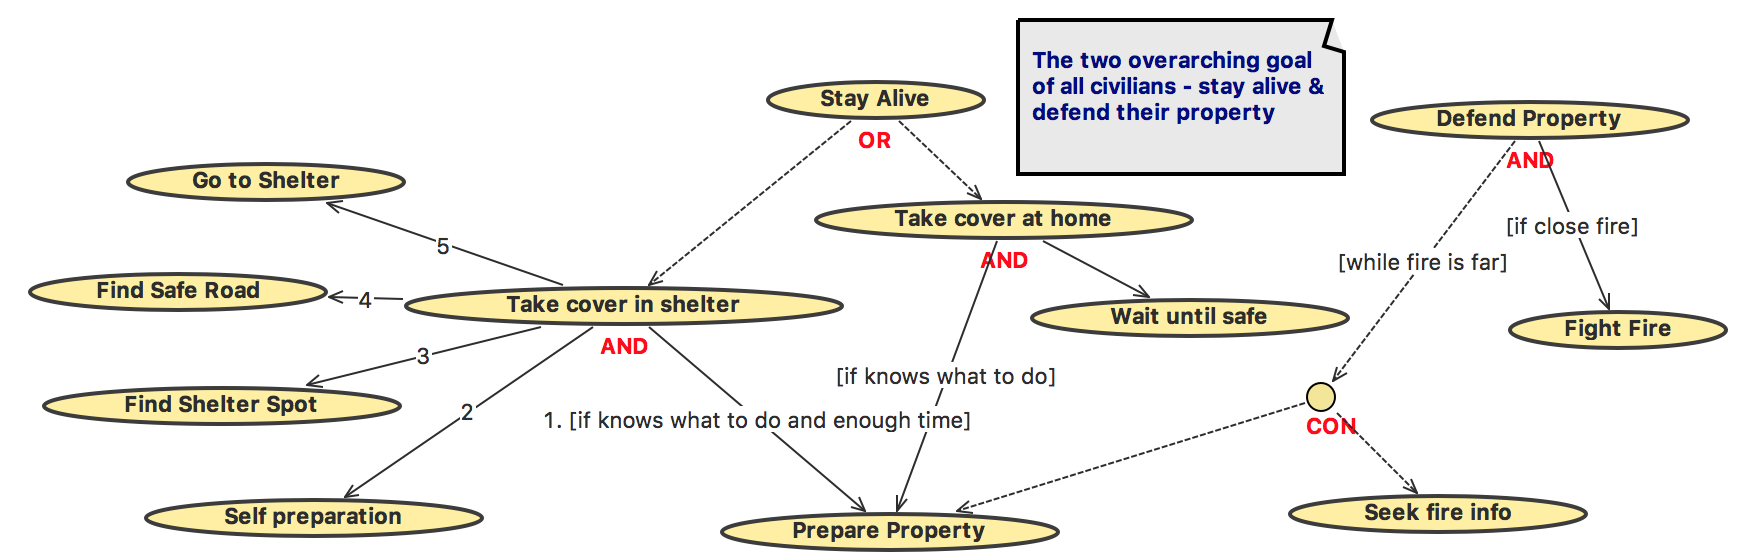
\includegraphics[scale=0.4]{GoalOverview.png}
						\caption{\label{fig:goal-overview}Goal overview for Pedestrian (civilians): decomposition of 2 main high-level goals,
						\textquotedblleft Stay Alive\textquotedblright and \textquotedblleft Defend Property\textquotedblright.}
					\end{center}
				\end{figure}

			\subsubsection{Role overview}

				The role overview diagram is used in order to associate the different roles for each agent.
				The figure \ref{fig:agent-role-overview} shows the 6 profiles of behaviours identified by Rhodes\cite{rhodes2014}
				from the witness statements. An agent can use only one role at the same time but can change over time.

				\begin{figure}
					\begin{center}
						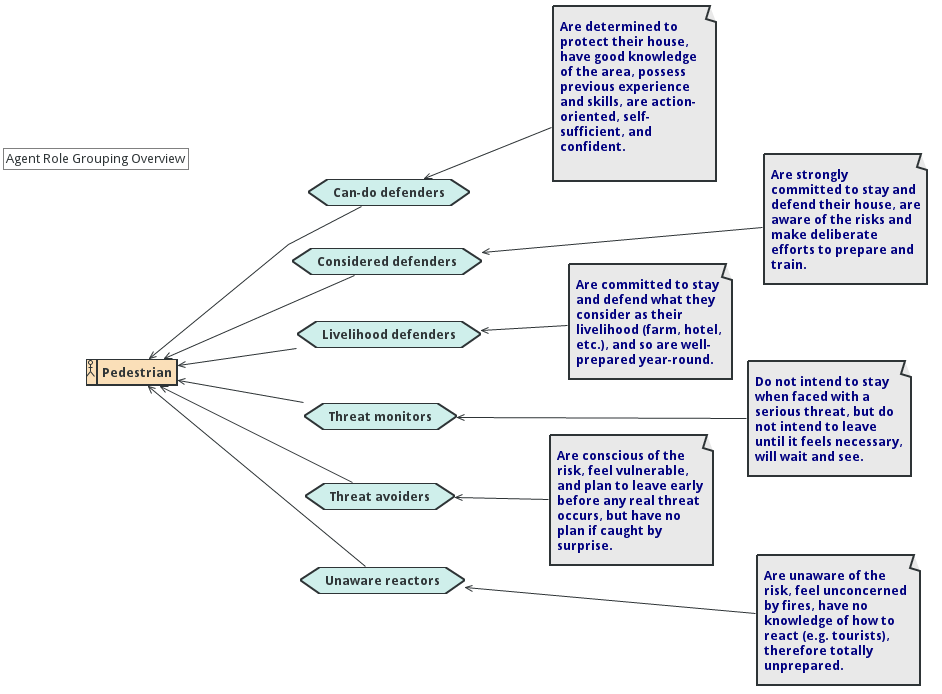
\includegraphics[scale=0.4]{Agent-role-grouping-overview.png}
						\caption{\label{fig:agent-role-overview} Agent role overview for Pedestrian.}
					\end{center}
				\end{figure}

			\subsubsection{System overview}

				The system overview (figure \ref{fig:system-overview}) allows to represent the relations between each percept (input) and related actions (output) of
				an agent (can have several agent). This diagram captures the interactions between the agents via protocols. In our
				case we have only one agent.

				\begin{figure}
					\begin{center}
						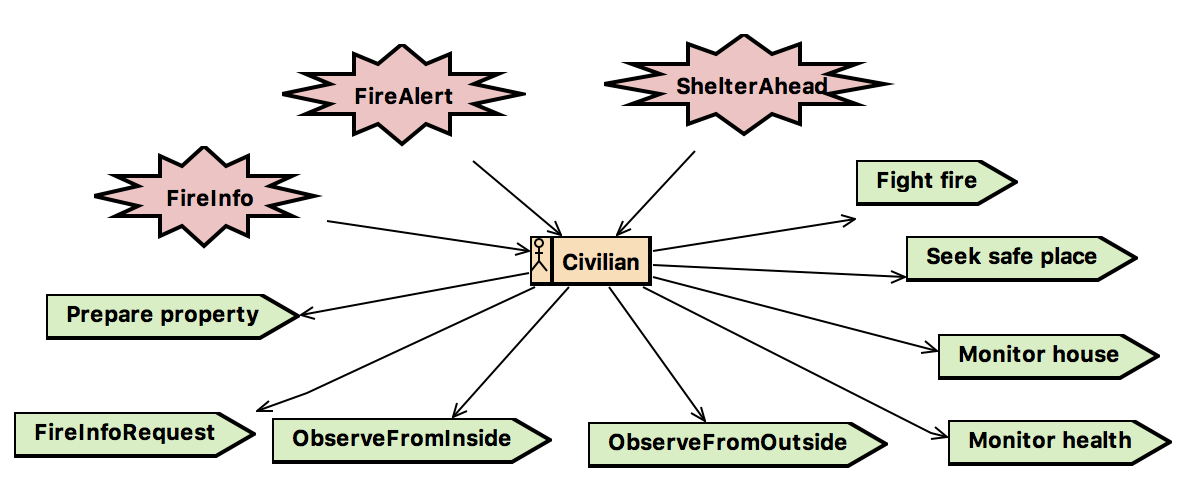
\includegraphics[scale=0.4]{SystemOverview.png}
						\caption{\label{fig:system-overview} System overview.}
					\end{center}
				\end{figure}

			\subsubsection{Agent overview}

				This diagram allows to make an overview of an agent with the associated capabilities and plans used to achieve
				their goals. The percept (input) and plan can be linked to one or several capacities. The agent can use only one of
				them at the same time. The figure \ref{fig:agent-overview} shows the overview of the Pedestrian agent with the
				related percepts and plans relevant to each capability.

				\begin{figure}
					\begin{center}
						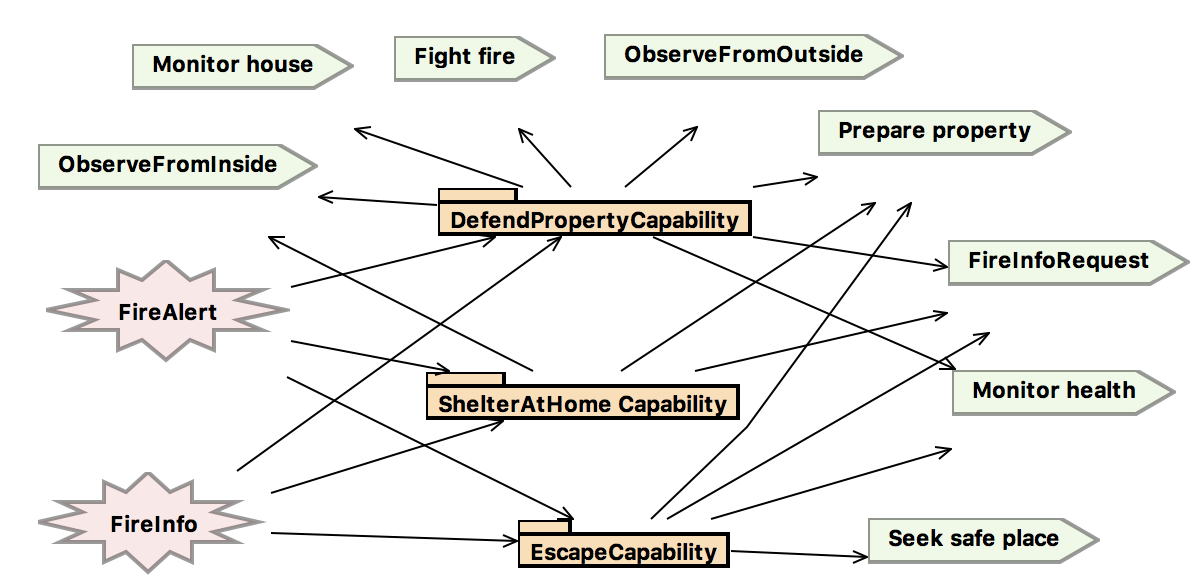
\includegraphics[scale=0.4]{Civillian-AgentOverview.png}
						\caption{\label{fig:agent-overview} Agent Overview, contains the capabilities of a Pedestrian (civilian) agent.}
					\end{center}
				\end{figure}

			\subsubsection{Capability overview}

				The capability overview represents the details of plans and sub-goals related to a specific capability. The figure \ref{fig:capability-overview}
				shows the details of the \textit{Defend property} capability. It shows as well the flow of activities and specifies the required data elements.
				For example, the \textquotedblleft\textit{Fire Data}\textquotedblright ~is read by the \textquotedblleft\textit{Defend Property}\textquotedblright ~plan
				and is written by the \textquotedblleft\textit{Observe Surroundings}\textquotedblright ~and \textquotedblleft\textit{Contact Fire Station}\textquotedblright ~plan.

				\begin{figure}
					\begin{center}
						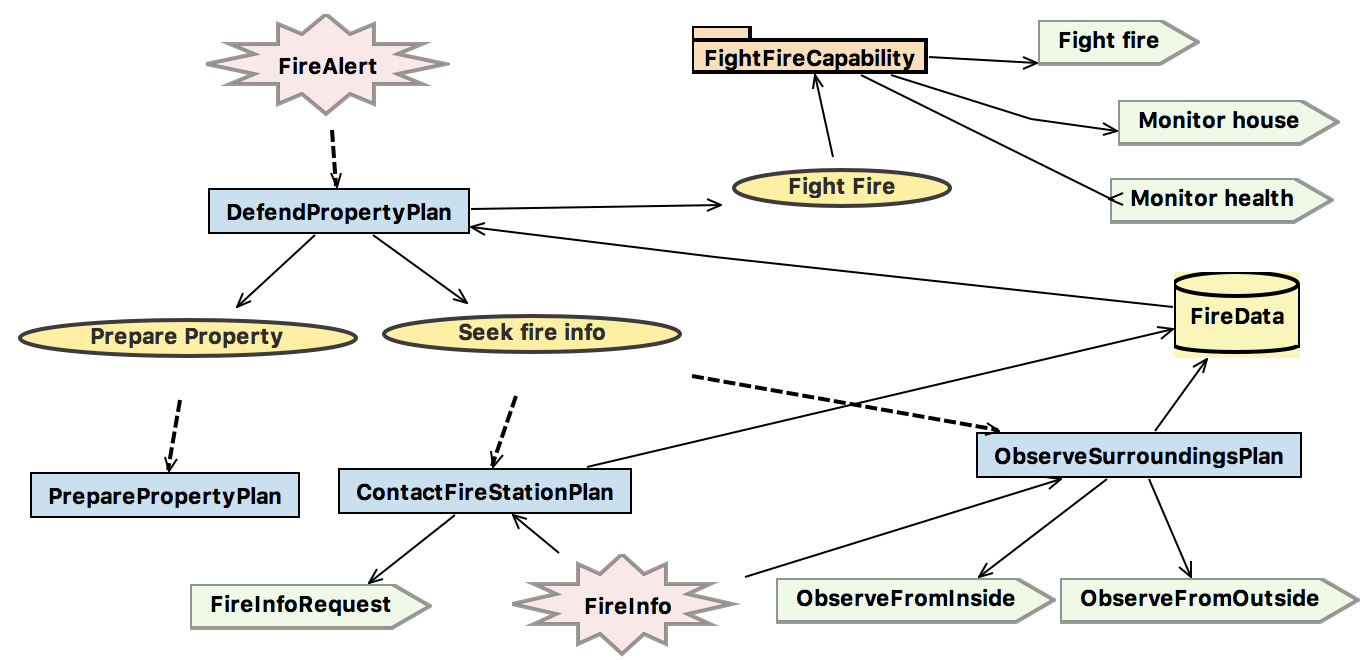
\includegraphics[scale=0.4]{CapabilityOverview.png}
						\caption{\label{fig:capability-overview} Description of the \textquotedblleft Defend Property \textquotedblright ~capability.}
					\end{center}
				\end{figure}

			\subsubsection{Plan diagrams}

				The plan diagrams are used in order to describe the plans (kind of UML activity diagram). A plan can be triggered by external
				percepts or goals, and is composed of several steps which can be sequential or concurrent. A Step can be atomic actions
				(external), activities (internal processes like \textquotedblleft write data\textquotedblright) or sub-goals.
				The figure \ref{fig:plan} shows the description of the \textquotedblleft\textit{Defend Property}\textquotedblright ~plan. This plan is triggered by the
				\textquotedblleft\textit{Fire Alert}\textquotedblright ~percept, and then uses \textquotedblleft\textit{Prepare Property}\textquotedblright ~and
				\textquotedblleft\textit{Seek Information}\textquotedblright ~goals concurrently. According to the consulted data (\textit{Fire Data}), the agent
				waits for fire to be close enough in order to use the \textquotedblleft\textit{Fight Fire}\textquotedblright ~goal.

				\begin{figure}
					\begin{center}
						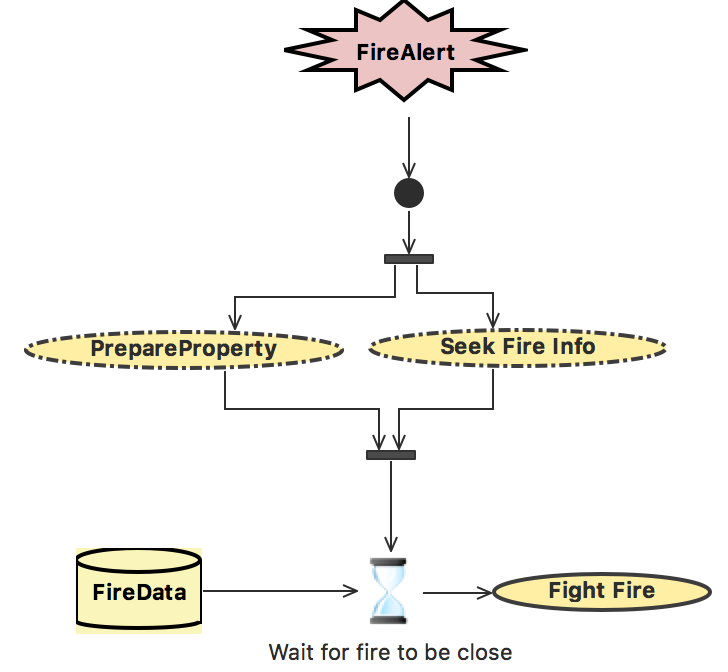
\includegraphics[scale=0.4]{plan.png}
						\caption{\label{fig:plan} Description of the \textquotedblleft Defend Property \textquotedblright plan.}
					\end{center}
				\end{figure}

	\section{GIS \& Agent-based Modelling Architecture}
		GIS \& Agent-based Modelling Architecture (GAMA) is an open source platform for modelling and simulations.
		It allows to build multi-agent systems into a spatial environment.
		Widely used, his developers community is active and is regularly improving the software. It allows scientists to use GIS data in simulation such as OpenStreetMap (OSM) with provide a fast way to build a precise mapping environment to the simulation. Furthermore, Gama has the advantage to make scalable simulations and to use a very simple and high level programming language called GAML\cite{gamawebsite,caillou2015,taillandier2016}.

		\subsection{GAML}

			\textbf{GA}MA \textbf{M}odeling \textbf{L}anguage also known as GAML is an agent-oriented language made from the necessity to have an easy language for non-computer scientists.
			Based on object-oriented languages like JAVA or Smalltalk, GAML is very close to agent-based modelling languages such as for example NetLogo. however, GAML has some additions like the
			inheritance, type safety or multi-level agency and provides a set of different behavioural architectures for programming agents.
			Althrough GAML is a programming language, the syntax was made in order to have a short learning curve and allow scientists to use GAMA in a short time.
			\paragraph{}
			The first step is to define a \textit{model species} (global model) which will include later the \textit{model agent} (the simulation), \textit{micro-species} and the \textit{experiment plans}.

			\subsubsection{Basic model structure}

				The \textbf{models} are the specifications of the simulations which can be controlled during an \textit{experiment} called also \textit{experiment plans}.

				\paragraph{}
				\underline{\textbf{Model Header}}
				\paragraph{}
				\begin{lstlisting}[mathescape,caption=Header model syntax.,label=code:header]
$\textcolor{purple}{model}$ name_of_the_model

$\textcolor{ForestGreen}{\text{// inclusion of files}}$
$\textcolor{purple}{import}$ $\textcolor{Cerulean}{"relative\_path\_to\_a\_model\_file"}$ [$\textcolor{purple}{as}$ model_identifier]

$\textcolor{purple}{global}$ {
  $\textcolor{ForestGreen}{\text{// Definition of [global attributes] (Global Species \#declaration)}}$
  $\textcolor{ForestGreen}{\text{//\ \ \ \ \ \ \ \ \ \ \ \ \ \ \ \ \ \ \ \ \ \ [actions and behaviors] (Defining Actions And Behaviors)}}$
}
				\end{lstlisting}

				A model must begin with the declaration of the name of the model by using the keyword \textbf{model} followed by the name.
				This name is used for building the name of the model species from which the simulations will be instantiated.
				The user can as well import existing file(s) using \textbf{import} and rename it with an alias with \textbf{as} (optional).
				The imported files will be merged in the model as \textit{micro-models}. The global species declaration is made through
				the \textbf{global} block declaration which contains the description of the \textit{model species}. Notice that the import
				and global declaration is not mandatory.

				\paragraph{}
				\underline{\textbf{Species}}
				\paragraph{}

				\begin{lstlisting}[mathescape,caption=Species declaration.,label=code:species]
$\textcolor{purple}{global}$ {

  $\textcolor{ForestGreen}{\text{// definition of global attributes, actions, behaviors. Accessible by all species}}$

  [...]

  $\textcolor{purple}{species}$ species_name [skills, control, schedules, ...] {
    ...
  }
}
				\end{lstlisting}

				Species provide a set of \textit{attributes} (what they know), \textit{actions} (what they can do),
				\textit{behaviors} (what they actually do) and also specifies properties of their population.
				The declaration of species is done with the keyword \textbf{species}. It is possible as well to define some optional
				descriptions to the species like \textbf{skills} (driving, moving, ...), \textbf{controls} (define the agent architecture type) or
				define some rules for the scheduler with \textbf{schedules}. A species can inherit its proprieties from another species called
				\textit{parent-species} or be included in another one (\textit{micro-species}). Species are used in order to define the agents.

				\paragraph{}
				\underline{\textbf{Experiment}}
				\paragraph{}

				An experiment is defined by the keywork \textbf{experiment} followed by the name of the experiment and the type (gui or batch).
				An gui experimentation allows to run one simulation per launch with the possibility to add visual output to interpret the results.
				In contrary of the gui type, the batch type is used in order to run the simulation severals times usually with graphics or data output.

				\begin{lstlisting}[mathescape,caption=Experiment declaration.,label=code:experiment]
$\textcolor{purple}{experiment}$ experiment_name $\textcolor{purple}{type}$: $\textcolor{Cerulean}{gui}$ (or $\textcolor{Cerulean}{batch}$) {

  $\textcolor{ForestGreen}{\text{// Experiments parameters which can be manipulated by the user}}$
  $\textcolor{purple}{parameter}$ $\textcolor{Cerulean}{\text{"Parameter's description"}}$ $\textcolor{Maroon}{var}$: variable_name [min, max, init, category];

  $\textcolor{purple}{output}$ {
    $\textcolor{purple}{display}$ display_name {
    }
    [monitor statements]
    [file statements]
  }
}
				\end{lstlisting}

		\subsubsection{BDI}

			This part will present the BDI implementation syntax through a simple example (see listing \ref{code:bdi}).
			The aim of this simulation will be to make a dummy BDI agent who will first take a look around its place and try to find fires in a radius area
			that we will call \textit{perception\_area}. After what, the agent will fight the fire if it enters the \textit{defense\_radius} area which correponds
			to the area where the agent thinks necessary to fight the fire.
			The \textbf{fire} will not be described in this part but has for goal to grow and burn all elements around.
			The first step is to define a new \textbf{species} which is called \textit{civilian} in this example. After the declaration of the species, we add
			the skill \textit{moving} using the keyword \textbf{skills} and of course we specify that we want a BDI agent by defining the \textbf{control} with
			\textit{simple\_bdi}.

			\begin{lstlisting}[mathescape,caption=BDI agent declaration.,label=code:bdi]
$\textcolor{purple}{species}$ civilian $\textcolor{Maroon}{skills}$:[$\textcolor{Cerulean}{moving}$] $\textcolor{Maroon}{control}$: $\textcolor{Cerulean}{simple\_bdi}$ {...}
			\end{lstlisting}

			Now, we have a new BDI agent which has the possibility to move. We can now define the required attributes such as the \textit{perception\_area} and the \textit{defense\_area}
			which will be used later. The declaration of variables is similar to a standard language such as in JAVA, C++, C ... In our case, we need a \textbf{float} or \textbf{integer} value in order to represent
			the radius areas. Moreover, we add an attribute to store known fires represented by a \textbf{list} of \textit{fire}. (see listing \ref{code:attribute})

			\begin{lstlisting}[mathescape,caption=Attributes declaration.,label=code:attribute]
$\textcolor{purple}{float}$ perception_radius <- $\textcolor{gray}{10.0}$;
$\textcolor{purple}{float}$ defense_radius <- $\textcolor{gray}{3.0}$;
$\textcolor{purple}{List}$<$\textcolor{Cerulean}{fire}$> known_fires;
			\end{lstlisting}

			The next step is to define the \textbf{predicates} (see listing \ref{code:perception}). The civilian agent has two predicates, the first one is the indication that the \textit{fire started},
			and the last one will be use in order to define if the agent want to \textit{protect its property}.

			\begin{lstlisting}[mathescape,caption=Predicates declaration.,label=code:perception]
$\textcolor{purple}{predicate}$ fire <- $\textcolor{PineGreen}{new\_predicate}$($\textcolor{Cerulean}{\text{"Fire started"}}$); $\textcolor{ForestGreen}{\text{// the agent believe that the fire started}}$
$\textcolor{purple}{predicate}$ protect_property <- $\textcolor{PineGreen}{new\_predicate}$($\textcolor{Cerulean}{\text{"Protect property"}}$); $\textcolor{ForestGreen}{\text{// the agent desire to fight against the fire}}$
			\end{lstlisting}

			We have created a new agent with some attributes and predicates. Now, we will see how to use these parameters in order to get a smarter agent. Indeed, the agent requires to have some instructions in order to
			know what to do according to the situation. To make this instructions, we will make a basic scenario and add little by little the required instructions.
			First we need to initialise the agent with an \textbf{init} block. In this block, we will define the initial agent's status and add the desire to protect its property.
			The keyword \textbf{do} will give an order to the agent which is to add the desire (\textbf{add\_desire}) to \textit{protect its property}.

			\begin{lstlisting}[mathescape,caption=Initialisation of the agent.,label=code:bdi]
$\textcolor{purple}{init}$ {
  $\textcolor{purple}{do}$ $\textcolor{PineGreen}{add\_desire}$($\textcolor{Cerulean}{protect\_property}$);
}
			\end{lstlisting}

			Let's suppose that the fire is started, we want the agent to take a look around its current position in order to detect potential fires. To do that, we need to add a \textbf{perception} with the \textbf{target} set on the
			\textit{fire}. Moreover, in order to make the simulation more realist, we can define a radius where the agent will not be able to see fires outside it. Thus, we use keyword \textbf{in} with the \textit{perception\_area} attribute
			previously declared (listing \ref{code:attribute}). The result of the perception will trigger the belief that the fire is indeed started.

			\begin{lstlisting}[mathescape,caption=Perceptions declaration.,label=code:bdi]
$\textcolor{purple}{perceive}$ $\textcolor{Maroon}{target}$:$\textcolor{Cerulean}{fire}$ $\textcolor{Maroon}{in}$:$\textcolor{Cerulean}{perception\_radius}$ {
  $\textcolor{purple}{add}$ self $\textcolor{Maroon}{to}$: myself.$\textcolor{Cerulean}{known\_fires}$; $\textcolor{ForestGreen}{\text{// self represent the current target and myself the agent}}$
  $\textcolor{purple}{ask}$ myself {
    $\textcolor{purple}{do}$ $\textcolor{PineGreen}{add\_belief}$($\textcolor{Cerulean}{fire}$);
  }
}
			\end{lstlisting}

			Let's assume now that the fire is close to the agent position, it believes that the fire is started and has the desire
			to defend its property. To satisfy his desire, the agent can use a plan. In order to create a new plan we
			use the keyword \textbf{plan} followed by the name of the plan (here \textit{fight\_fire}). After the plan declaration, we need
			to link it with the associated \textbf{intention} \textit{protect\_property}. This declaration means that this plan is used
			in order to satisfy the specified intention which is here \textit{defend its property}. Furthermore, we need to specify that the plan cannot be used without
			fire at proximity of the agent position. This condition can be expressed with the keyword \textbf{when} followed by the condition.
			\newline
			The conditions are the following:
			\begin{itemize}
				\item A known fire must be present in the defense area: To write this condition we need first to get the list of fires in
				the area using the keyword \textbf{at\_distance}  which will provide a list of fires in the defense radius (right part of the keyword) among the
				known fires (left part). After getting the list of fires, we check if the list is empty (no known fire at proximity) or not using the
				negation \textbf{not} and the \textbf{empty} function.
				\item The last condition is to check if the agent believes that the fire is started. If the agent does not believe that the fire is
				currently started, it will think then it is useless to fight the fire without fire at proximity (which makes sense). This verification is
				made by the function \textbf{has\_belief} which will be true if the agent at this moment believes the predicate between the parenthesis.
			\end{itemize}

			\begin{lstlisting}[mathescape,caption=Plans declaration.,label=code:bdi]
$\textcolor{purple}{plan}$ fight_fire
  $\textcolor{Maroon}{intention}$: $\textcolor{Cerulean}{protect\_property}$
  $\textcolor{Maroon}{when}$: (
          $\textcolor{purple}{not}$ $\textcolor{PineGreen}{empty}$($\textcolor{Cerulean}{known\_fires}$ $\textcolor{PineGreen}{at\_distance}$ $\textcolor{Cerulean}{defense\_radius}$)
          $\textcolor{Maroon}{and}$ $\textcolor{PineGreen}{has\_belief}$($\textcolor{Cerulean}{fire}$)
        )
  $\textcolor{Maroon}{finished\_when}$: $\textcolor{PineGreen}{empty}$($\textcolor{Cerulean}{known\_fires}$ $\textcolor{PineGreen}{at\_distance}$ $\textcolor{Cerulean}{defense\_radius}$)
{
  $\textcolor{purple}{ask}$ $\textcolor{Cerulean}{known\_fires}$ $\textcolor{PineGreen}{at\_distance}$ ($\textcolor{Cerulean}{defense\_radius}$)
  {
    $\textcolor{purple}{float}$ FightingEffect <- rnd(4.0); $\textcolor{PineGreen}{\text{// The FightingEffect is a random value between 0 and 4}}$
    intensity <- intensity - fightingEffect;
  }
}
			\end{lstlisting}

			The last thing to define is the content of the plan. In order to simulate the fire fighting effect, we will generate a random value corresponding to
			the effect of the action (here a random value between 0 and 4) on the fire which will be stored in a variable called \textit{fightingEffect}. After what,
			we just have to reduce the intensity of all known fires in the defense radius ($\textcolor{purple}{ask}$ $\textcolor{Cerulean}{known\_fires}$ $\textcolor{PineGreen}{at\_distance}$ ($\textcolor{Cerulean}{defense\_radius}$))
			by the value of the variable previously created. The final result of this agent is represented in the listing \ref{code:bdi}.

			\begin{lstlisting}[mathescape,caption=Exemple of BDI agent.,label=code:bdi]
$\textcolor{purple}{species}$ civilian $\textcolor{Maroon}{skills}$:[$\textcolor{Cerulean}{moving}$] $\textcolor{Maroon}{control}$: $\textcolor{Cerulean}{simple\_bdi}$ {
  $\textcolor{purple}{float}$ perception_radius <- $\textcolor{gray}{10.0}$;
  $\textcolor{purple}{float}$ defense_radius <- $\textcolor{gray}{3.0}$;
  $\textcolor{purple}{List}$<$\textcolor{Cerulean}{fire}$> known_fires;

  $\textcolor{ForestGreen}{\text{// Predicates}}$
  $\textcolor{purple}{predicate}$ fire <- $\textcolor{PineGreen}{new\_predicate}$($\textcolor{Cerulean}{\text{"Fire started"}}$); $\textcolor{ForestGreen}{\text{// the agent believe that the fire started}}$
  $\textcolor{purple}{predicate}$ protect_property <- $\textcolor{PineGreen}{new\_predicate}$($\textcolor{Cerulean}{\text{"Protect property"}}$); $\textcolor{ForestGreen}{\text{// the agent desire to fight against the fire}}$

  $\textcolor{ForestGreen}{\text{// Agent initialisation}}$
  $\textcolor{purple}{init}$ {
    $\textcolor{purple}{do}$ $\textcolor{PineGreen}{add\_desire}$($\textcolor{Cerulean}{protect\_property}$);
  }

  $\textcolor{ForestGreen}{\text{// Perceptions}}$
  $\textcolor{purple}{perceive}$ $\textcolor{Maroon}{target}$:$\textcolor{Cerulean}{fire}$ $\textcolor{Maroon}{in}$:$\textcolor{Cerulean}{perception\_radius}$ {
    $\textcolor{purple}{add}$ self $\textcolor{Maroon}{to}$: myself.$\textcolor{Cerulean}{known\_fires}$; $\textcolor{ForestGreen}{\text{// self represent the current target and myself the agent}}$
    $\textcolor{purple}{ask}$ myself {
      $\textcolor{purple}{do}$ $\textcolor{PineGreen}{add\_belief}$($\textcolor{Cerulean}{fire}$);
    }
  }

  $\textcolor{ForestGreen}{\text{// Plans}}$
  $\textcolor{purple}{plan}$ fight_fire
    $\textcolor{Maroon}{intention}$: $\textcolor{Cerulean}{protect\_property}$
    $\textcolor{Maroon}{when}$: (
            $\textcolor{purple}{not}$ $\textcolor{PineGreen}{empty}$($\textcolor{Cerulean}{known\_fires}$ $\textcolor{PineGreen}{at\_distance}$ $\textcolor{Cerulean}{defense\_radius}$)
            $\textcolor{Maroon}{and}$ $\textcolor{PineGreen}{has\_belief}$($\textcolor{Cerulean}{fire}$)
          )
    $\textcolor{Maroon}{finished\_when}$: $\textcolor{PineGreen}{empty}$($\textcolor{Cerulean}{known\_fires}$ $\textcolor{PineGreen}{at\_distance}$ $\textcolor{Cerulean}{defense\_radius}$)
  {
    $\textcolor{purple}{ask}$ $\textcolor{Cerulean}{known\_fires}$ $\textcolor{PineGreen}{at\_distance}$ ($\textcolor{Cerulean}{defense\_radius}$)
    {
      $\textcolor{purple}{float}$ FightingEffect <- rnd(4.0); $\textcolor{PineGreen}{\text{// The fightingEffect is a random value between 0 and 4}}$
      intensity <- intensity - fightingEffect;
    }
  }
}
			\end{lstlisting}

		\subsubsection{Finite State Machine (FSM)}

			This part describe briefly the FSM architecture of GAML. The following example is based on the ant toy model available on GAMA.
			In this model, the ants have for objective to find food and bring it back.
			The declaration of the agent is similar to the BDI declaration but with the keyword \textbf{fsm} instead of \textbf{simple\_bdi}.
			An ant has for \textit{attribute} a boolean value which determines if the ant currently has food or not.

			\begin{lstlisting}[mathescape,caption=Ant attribute.,label=code:ant_attribute]
$\textcolor{purple}{bool}$ hasFood <- $\textcolor{gray}{false}$;
			\end{lstlisting}

			To allow ants to have the possibility to pick or drop food, we can for instance use the \textbf{action} which is
			equivalent to a process or function. The pick function will switch the boolean value to \textit{true} in contrary of
			drop which will switch it back to false.

			\begin{lstlisting}[mathescape,caption=Pick action.,label=code:pick]
$\textcolor{PineGreen}{\text{//Action to pick the food}}$
$\textcolor{purple}{action}$ pick {
  hasFood <- $\textcolor{gray}{true}$;
}

$\textcolor{PineGreen}{\text{//Action to drop the food}}$
$\textcolor{purple}{action}$ drop {
  hasFood <- $\textcolor{gray}{false}$;
}
			\end{lstlisting}

			The next step is to define the states. The declaration of the state is made by the keyword \textbf{state}.
			For example, we want define the initial step of this simulation, which consist in searching randomly in the
			area some food or a road made previously by another ant which has discovered food. We create a new state with
			the name \textit{wandering} and add after the name the keyword \textbf{initial} set to \textit{true}.
			This option defines the state as the initial state. We need now to tell that the ant must search in the area.
			For that, we use the order keyword \textbf{do} following by the order \textbf{wander} and define an \textbf{amplitude}
			set to 120 units from the current ant location for instance. Let's now assume that the ant discovers food.
			We need to change the state of the ant from \textit{wandering} to the next state \textit{carryingFood}. To make the
			transition, we first use \textbf{transition} followed by the name of the new state (here \textit{carryingFood}) and with
			the condition of the transition (place.food \textgreater 0) which represents whether the place contains food (0 means that there is no food).

			\begin{lstlisting}[mathescape,caption=Initial state of the FSM.,label=code:initstate]
$\textcolor{PineGreen}{\text{//initial state of the ant that will make it wander until it finds food or a road}}$
$\textcolor{purple}{state}$ wandering $\textcolor{Maroon}{initial}$: $\textcolor{gray}{true}$ {
  $\textcolor{purple}{do}$ $\textcolor{Cerulean}{wander}$ $\textcolor{Maroon}{amplitude}$:$\textcolor{gray}{120}$; $\textcolor{PineGreen}{\text{// Search randomly in a radius of 120 units around the current position}}$
  $\textcolor{purple}{transition}$ $\textcolor{Maroon}{to}$: $\textcolor{Cerulean}{carryingFood}$ $\textcolor{Maroon}{when}$: $\textcolor{Cerulean}{place}$.$\textcolor{Cerulean}{food}$ > $\textcolor{gray}{0}$ {
    $\textcolor{purple}{do}$ $\textcolor{Cerulean}{pick}$;
  }
  $\textcolor{purple}{transition}$ $\textcolor{Maroon}{to}$: $\textcolor{Cerulean}{followingRoad}$ $\textcolor{Maroon}{when}$: $\textcolor{Cerulean}{place}$.$\textcolor{Cerulean}{road}$ > $\textcolor{gray}{0.05}$;
}
			\end{lstlisting}

			Before bringing back the food, the ant must make a road for the other ants in order to show them the location of the food.
			In order to do that, we can use the keyword \textbf{reflex}. The reflex is a process which will be executed each cycle of
			the simulation if the condition (optional) is true. In our case, the condition is that the ant must carry food (defined by the boolean
			\textit{hasFood}).

			\begin{lstlisting}[mathescape,caption=Finite State Machine exemple.,label=code:fsm]
$\textcolor{PineGreen}{\text{//Reflex to allow the diffusion of the road of pheromon by putting pheromon inside a cell}}$
$\textcolor{purple}{reflex}$ diffuse_road $\textcolor{Maroon}{when}$: $\textcolor{Cerulean}{hasFood}$ = $\textcolor{gray}{true}$ {
  $\textcolor{PineGreen}{ant\_grid}$($\textcolor{Cerulean}{location}$).$\textcolor{Cerulean}{road}$ <- $\textcolor{PineGreen}{ant\_grid}$($\textcolor{Cerulean}{location}$).$\textcolor{Cerulean}{road}$ + $\textcolor{gray}{100.0}$;
}
			\end{lstlisting}

			The final step is to create the other states which are: following the road (\textit{followingRoad}) and carrying food (\textit{carryingFood}).
			Finally, we obtain the following result :

			\begin{lstlisting}[mathescape,caption=Finite State Machine exemple.,label=code:fsm]
$\textcolor{PineGreen}{\text{//Species ant that will move and follow a final state machine}}$
$\textcolor{purple}{species}$ ant $\textcolor{Maroon}{skills}$: [$\textcolor{Cerulean}{moving}$] $\textcolor{Maroon}{control}$: $\textcolor{Cerulean}{fsm}$ {
  $\textcolor{purple}{bool}$ hasFood <- $\textcolor{gray}{false}$;

  $\textcolor{PineGreen}{\text{//Reflex to allow the diffusion of the road of pheromon by putting pheromon inside a cell}}$
  $\textcolor{purple}{reflex}$ diffuse_road $\textcolor{Maroon}{when}$: $\textcolor{Cerulean}{hasFood}$ = $\textcolor{gray}{true}$ {
    $\textcolor{PineGreen}{ant\_grid}$($\textcolor{Cerulean}{location}$).$\textcolor{Cerulean}{road}$ <- $\textcolor{PineGreen}{ant\_grid}$($\textcolor{Cerulean}{location}$).$\textcolor{Cerulean}{road}$ + $\textcolor{gray}{100.0}$;
  }

  $\textcolor{PineGreen}{\text{//Action to pick the food}}$
  $\textcolor{purple}{action}$ pick {
    hasFood <- $\textcolor{gray}{true}$;
  }

  $\textcolor{PineGreen}{\text{//Action to drop the food}}$
  $\textcolor{purple}{action}$ drop {
    hasFood <- $\textcolor{gray}{false}$;
  }

  $\textcolor{PineGreen}{\text{//initial state of the ant that will make it wander until it finds food or a road}}$
  $\textcolor{purple}{state}$ wandering $\textcolor{Maroon}{initial}$: $\textcolor{gray}{true}$ {
    $\textcolor{purple}{do}$ $\textcolor{Cerulean}{wander}$ $\textcolor{Maroon}{amplitude}$:$\textcolor{gray}{120}$; $\textcolor{PineGreen}{\text{// Search randomly in a radius of 120 units around the current position}}$
    $\textcolor{purple}{transition}$ $\textcolor{Maroon}{to}$: $\textcolor{Cerulean}{carryingFood}$ $\textcolor{Maroon}{when}$: $\textcolor{Cerulean}{place}$.$\textcolor{Cerulean}{food}$ > $\textcolor{gray}{0}$ {
      $\textcolor{purple}{do}$ $\textcolor{Cerulean}{pick}$;
    }
    $\textcolor{purple}{transition}$ $\textcolor{Maroon}{to}$: $\textcolor{Cerulean}{followingRoad}$ $\textcolor{Maroon}{when}$: $\textcolor{Cerulean}{place}$.$\textcolor{Cerulean}{road}$ > $\textcolor{gray}{0.05}$;
  }

  $\textcolor{PineGreen}{\text{//State to carry food to the nest once it has been found}}$
  $\textcolor{purple}{state}$ carryingFood {
    $\textcolor{purple}{do}$ $\textcolor{Cerulean}{goto}$ $\textcolor{Maroon}{target}$: $\textcolor{Cerulean}{center}$;
    $\textcolor{purple}{transition}$ $\textcolor{Maroon}{to}$: $\textcolor{Cerulean}{wandering}$ $\textcolor{Maroon}{when}$: $\textcolor{Cerulean}{place}$.$\textcolor{Cerulean}{isNestLocation}$ {
      $\textcolor{purple}{do}$ $\textcolor{Cerulean}{drop}$;
    }
  }

  $\textcolor{PineGreen}{\text{//State to follow a pheromon road once it has been found}}$
  $\textcolor{purple}{state}$ followingRoad {
    location <- (self $\textcolor{PineGreen}{choose\_best\_place}$()) $\textcolor{Maroon}{as}$ $\textcolor{Cerulean}{point}$;
    $\textcolor{purple}{transition}$ $\textcolor{Maroon}{to}$: $\textcolor{Cerulean}{carryingFood}$ $\textcolor{Maroon}{when}$: $\textcolor{Cerulean}{place}$.$\textcolor{Cerulean}{food}$ > $\textcolor{gray}{0}$ {
      $\textcolor{purple}{do}$ $\textcolor{Cerulean}{pick}$;
    }
    $\textcolor{purple}{transition}$ $\textcolor{Maroon}{to}$: $\textcolor{Cerulean}{wandering}$ $\textcolor{Maroon}{when}$: ($\textcolor{Cerulean}{place}$.$\textcolor{Cerulean}{road}$ < $\textcolor{gray}{0.05}$);
  }
}
			\end{lstlisting}


			\section{From TDF to GAML}

				In this part we will explain who TDF diagrams can be used in order to produce GAML code. To illustrate this section,
				we will use the diagrams previously described in the section \ref{sec:tdf} and make the model of the senario \textit{Defend Property}.
				We assume that we already created an Pedestrian agent and there exist an fire implementation. We assume as well that each Pedestrian
				has a house which have to be defended.
				\paragraph{}
				To begin, the figure \ref{fig:analysis-overview} and \ref{fig:scenario} provide the global information about the senario we must
				create. The goal is composed of 2 percepts, 3 goals and 1 action.
				The figure \ref{fig:plan} and \ref{fig:goal-overview} provide more information about the progress of the scenario and about the different sub-goals.
				We know now that to achive the goal \textit{Defend Property} the agent need to \textit{fight the fire} if its close or to \textit{prepare its property}
				or to \textit{seek information} about the fire. Moreover, we can deduce from the diagram represented in the figure \ref{fig:goal-overview} the different predicates.

				\subsubsection{Predicate}

					According to the goal overview (figure \ref{fig:goal-overview}) and the plan description (figure \ref{fig:plan}), we can deduce that we need to create
					2 predicates. The first one is the predicate which will be used in order to represent the intention to protect the property (called \textit{protect\_property}).
					The second one is the trigger of the scenario \textit{fire\_position} which represents the acknowledgement of a fire position (see listing \ref{code:agent-predicate}).

					\begin{lstlisting}[mathescape,caption=Agent predicates.,label=code:agent-predicate]
$\textcolor{purple}{predicate}$ fire_position <- $\textcolor{PineGreen}{new\_predicate}$($\textcolor{Cerulean}{\text{"Know the fire position"}}$);
$\textcolor{purple}{predicate}$ protect_property <- $\textcolor{PineGreen}{new\_predicate}$($\textcolor{Cerulean}{\text{"Protect property"}}$);
					\end{lstlisting}

				\subsubsection{Percepts}

					As we have seen previously, the figure \ref{fig:capability-overview} informs us that the first percept (\textit{FireAlert}) is the trigger of the
					scenario and the second percept (\textit{FireInfo}) is the result of the information research about a fire. We know as well that its related to the fire position (see figure \ref{fig:scenario}).
					In order to create the perception \textit{FireAlert}, we create at first a \textquotedblleft\textit{perceive}\textquotedblright ~block with for target all \textit{fires}
					in the \textit{perception area}.
					The content of the perception is filling the agent's database about fire called \textit{known\_fires}, add the belief about the fire position and add the desire to protect the property.

					\begin{lstlisting}[mathescape,caption=Perception FireAlert.,label=code:percept-firealert]
$\textcolor{purple}{perceive}$ $\textcolor{Maroon}{target}$:$\textcolor{Cerulean}{fire}$ $\textcolor{Maroon}{in}$:$\textcolor{Cerulean}{perceptionArea}$ {
  $\textcolor{purple}{add}$ self $\textcolor{Maroon}{to}$: myself.$\textcolor{Cerulean}{known\_fires}$; $\textcolor{ForestGreen}{\text{// self represent the current target and myself the agent}}$
  $\textcolor{purple}{ask}$ myself {
    $\textcolor{purple}{do}$ $\textcolor{PineGreen}{add\_belief}$($\textcolor{Cerulean}{fire\_position}$);
    $\textcolor{purple}{do}$ $\textcolor{PineGreen}{add\_desire}$($\textcolor{Cerulean}{protect\_property}$);
  }
}
					\end{lstlisting}

				\subsubsection{Plans}

					The description of each plan are available on the capability overview (figure \ref{fig:capability-overview}) and the plan diagram (\ref{fig:plan}).
					For example the listing \ref{code:plan-prepare} correponds to the plan \textit{PrepareProperty}. This goal can be used if the agent are aware of the fire and
					if the fire is far enough to allows the agent to make some preparation of its property.

					\begin{lstlisting}[mathescape,caption=Plan PrepareProperty.,label=code:plan-prepare]
$\textcolor{purple}{plan}$ PrepareProperty
  $\textcolor{Maroon}{intention}$: $\textcolor{Cerulean}{protect\_property}$
  $\textcolor{Maroon}{when}$: (
          $\textcolor{PineGreen}{empty}$($\textcolor{Cerulean}{known\_fires}$ $\textcolor{PineGreen}{at\_distance}$ $\textcolor{Cerulean}{defense\_radius}$)
          $\textcolor{Maroon}{and}$ $\textcolor{PineGreen}{has\_belief}$($\textcolor{Cerulean}{fire\_position}$)
        )
{
  $\textcolor{purple}{do}$ $\textcolor{PineGreen}{HousePreparation}$;
}
					\end{lstlisting}

\chapter{Data description \label{chapter:data}}

	The goal of our study is to make a BDI multi-agent simulation of citizen behaviour during a bushfire.
  This study is principally based on related works, on witness statements from the Black Saturday\cite{witness} and from the last studies about Australian bushfires\cite{rhodes2014, adam2015}.
	\section{Witness statements}

		The witness statements are a good source of information about the peoples behaviour during this day.
		These witness statements show that there exist several behaviours and profiles. The first main difference is the awareness of the fire risk.
		The citizens who have made fire training at the CFA know about fire risks and have potentially more chance to know how to fight a fire.
		According to their priority, if they have a family to protect or if their house is very important (family house, livelihood ...)
		the person will have for first intention to leave or to protect their property or will simply wait to see if the fire is coming to their direction.
		Among people who want to stay, we can find two types of person. The first one want to protect their property but does not know how to fight fire and does not have equipped his house for that, these persons have a low danger aversion.
		The second type want to protect their property and is well prepared. The fact that they know how to fight a fire can produce two types of interpretation during a bushfire.
		A person who knows how to fire a fire can have a very high confidence in their skill and finally underestimate the intensity of the fire.
		However, some other people who wanted initially to fight the fire will change their mindset when they realised that the fire is too important in order to be extinguished.
		\paragraph{}
		Witness statements were used as well in order to make TDF digrams. An example with the following sentence:
		\begin{quote}
			\textquotedblleft While Gary was getting the fire pump ready, I checked the CFA website but I couldn't find anything that related to our district.\textquotedblright \cite{exell}
		\end{quote}

		This sentence show that before the fire was too close from the house, Gary made some preparation (\textit{Prepare Property}) and Sue was searching information with the radio (\textit{seek information}).
	\section{Profiles}

		A previous study shows there exist six archetypes of population behaviour. These archetypes describe some
		pattern such as the risk perception, attitudes, intentions, priority and behaviours\cite{rhodes2014, adam2015}:
		\begin{itemize}
			\item \textbf{Can do defenders}: They are self-sufficient, confident, practical and motivated to deal with the fire in order to protect
			his property. They have a good knowledge of the area, are experimented with fires and are aware of the risk. They rely on
			their own judgement and resources. They use official warnings but often rely on local sources and their own observations.
			\item \textbf{Considered defenders}: Although they know the related risk of the fire, they will make a conscious decision to protect
			their property. They spend time and ressources in order to deal with the fire. They are well connected in their community, are engaged
			with the fire agencies, participate in programs and seek information regularly. They are familiar with sources of warning but use their
			own observations to assess the situation.
			\item \textbf{Livelihood defender}: Defend their property which are their livelihood (farmer). Often long-term resident, experimented
			with the fire and will not give it up easily. They are motivated by the need to protect their livelihood. There are self-reliant, practical
			with a good local knowledge. They are well connected and are often volunteers in local brigades. They rely on the local knowledge and networks to
			get information about the threat and make their own judgement of the situation.
			\item \textbf{Threat monitor}: Does not intend to remain but they will not leave until they think it is necessary to leave. They remain
			in order to prepare their property and will not leave before the completion of their tasks, the proximity of fire, they perceive a danger,
			or advice from authorities. They are aware about the risk but try to balance the threat against their priorities. They do not have backup
			plans because they want to leave before it becomes dangerous.
			\item \textbf{Threat avoider}: Are aware of the risk and feel vulnerable. They leave before there is \textquotedblleft any source of danger \textquotedblright
			~or as soon as possible. They can have limited capability, responsibility for dependants, undefendable property or the fear of the threat.
			They support the emergency services but do not seek safety information because they think that leaving will solve the problem. They do various
			tasks before leaving such as moving important item from the property or make preparation in order to leave. They rely on the official
			warnings sources and leave if the authorities advise them to do so.
			\item \textbf{Unaware reactor}: Do not think they are leaving in a fire risk area because of the unfamilarity with the environment and risk
			and do not feel concerned. Even if they aknowledge about the environment risk which can occur in the area, they will not expect to be affected.
			They do not seek information about what to do, do not make or prepare plan. They have no idea of what they must do if fires occur and leave if
			they feel in danger or wait to see they really need to leave. They follow official advice to leave if they receive it but the presence of emergencies
			services have an influence to lead them to believe the threat is being managed.
		\end{itemize}

		\begin{table}
			\caption{Summary of profiles.}
			\begin{tabular}{|c|c|c|c|c|}
			  \hline
			  Profile & Experience/capacity & First intention & Determination & Danger aversion \\
			  \hline
			  Can do defenders & high & Defend & high & low\\
				\hline
			  Considered defenders & moderate & Defend & moderate & moderate\\
				\hline
				Livelihood defender & high & Defend & very high & very low\\
				\hline
				Threat monitor & moderate & Leave if close fire & low &  high\\
				\hline
				Threat avoider & low & Leave & low & very high\\
				\hline
				Unaware reactor & null & null & null & low\\
			  \hline
			\end{tabular}
		\end{table}

	\section{Statistics}

	The statistics used in this project have been made by the VBRC, these statistics contain essentially information about
	the damages caused by the fire during the Black Saturday (number of burnt buildings, number of dead, \dots). The most
	interesting statistics we can find are data about the causes of the death.

	The Professor John Handmer of RMIT University report the following results about the behaviour of the peoples
	who died during the Black Saturday\cite{stats2009}:
	\begin{itemize}
		\item 58\% had made no preparation either for staying and defending or for leaving early (\textit{Threat avoider}). Many of these peoples
		prepare to leave but was apparently awaiting a warning (\textit{Threat monitors}).
		\item 20\% intended to stay and defend and was well prepared (\textit{Can-do defenders}) and 14\% made limited preparation (\textit{Considered defenders}).
		\item The fire took by surprise 30\% of those who died.
		\item 24\% was unaware that they were in a bushfire risk area, 38\% did not seem to have a basic knowledge about what they should do in this situation (\textit{Unaware reactors}).
		\item 14\% were fleeing the fire at the time of their death (4\% by car and 10\% by foot).
		\item 69\% was \textquotedblleft passively sheltered$\textquotedblright$ inside a house or other building at time of their death (some of these tried to defend their property).
		\item 44\% was classed as \textquotedblleft vulnerable$\textquotedblright$ because of the age (less than 12 or more than 70 years old) or because
		they were suffering from an acute or chronic illness or disability (more detailsa bout the age and gender repartition on the figure \ref{fig:stats}).
		\item 32\% died of the peoples died on properties whose defendability was questionable.
	\end{itemize}

	\begin{figure}
		\begin{center}
			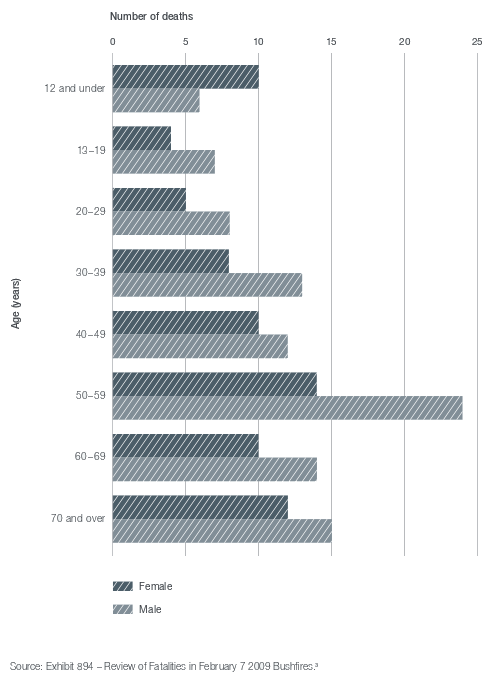
\includegraphics[scale=0.8]{stats2.png}
			\caption{
				\label{fig:stats} Those who died: Age and gender profile.
			}building)[13].
		\end{center}
	\end{figure}

\chapter{Implementation description}

	In order to make our simulation, we chose to use the GAMA software which provides a plug-in for BDI implementations with an extension
	of the GAML language \cite{caillou2015}. GAML has the advantage to be simple to use and to understand. The BDI implementation
	is based on a previous simulation written on GAMA which use an finite-state machine (figure \ref{fig:automaton}) for the agents
	reasoning \cite{adam2015}. The behaviour of agent in the finite state machine implementation is represented by 7 steps. The first
	step (initial step) is the \textit{Unaware} step. When the agent detect a fire, it switch from \textit{Unaware} to \textit{Aware indecisive}.
	The decision-making process is done by two random value (\textit{defendMotivation} and \textit{escapeMotivation}). The \textit{flip} function is used in order to
	generate a number between 0 and the value defined in parameter which corresponds to the probability to get a \textit{true} (boolean value). The higher value between
	these two flips determine if the agent chooses to defend or leave. This decision making process and the lack of flexibility is the biggest weakness of the finite state machine
	architecture. Indeed, an agent cannot change its strategy if the FSM does not make the transition explicitly. This is for this reason, the BDI architecture provides a real benefice in term of realism.
	The BDI implementation use the same environment and fire model.

	\begin{figure}
		\begin{center}
			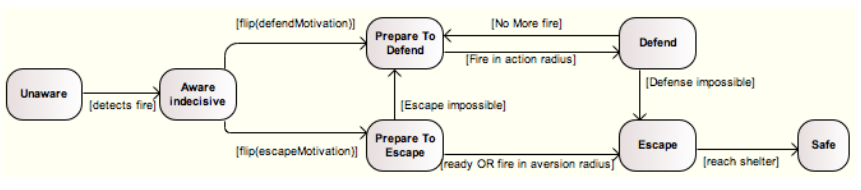
\includegraphics[scale=0.8]{automaton.png}
			\caption{\label{fig:automaton}Finite-state machine of the agent behaviour\cite{adam2015-2}.}
		\end{center}
	\end{figure}

	\begin{figure}
		\begin{center}
			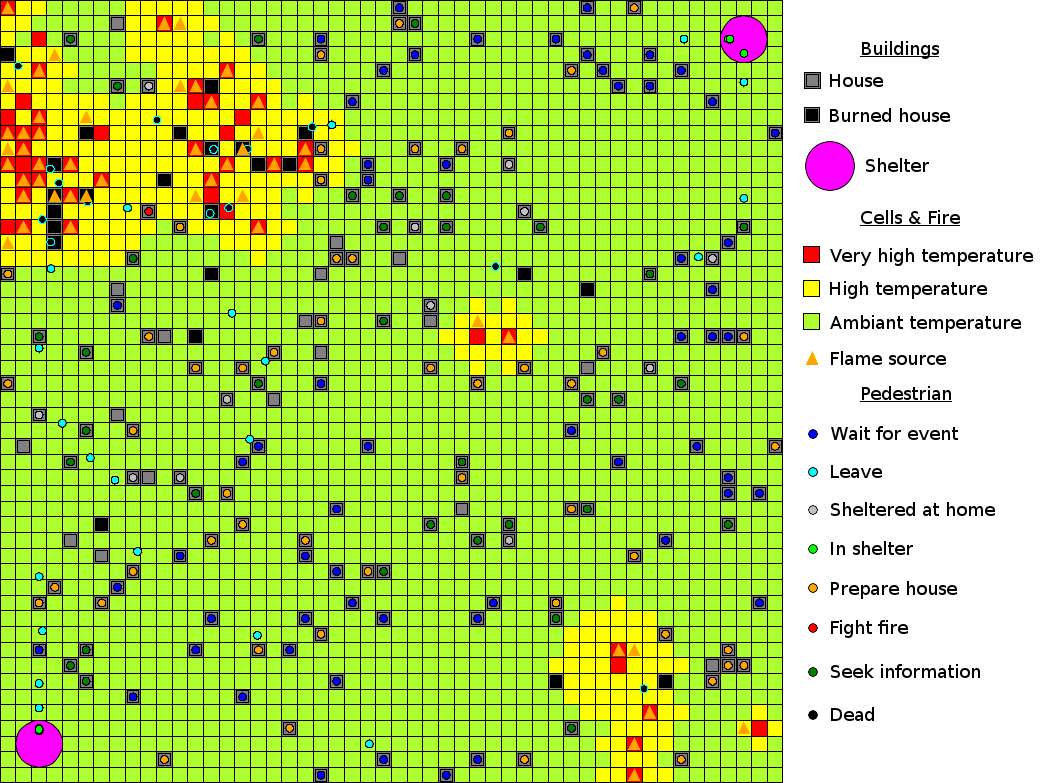
\includegraphics[scale=0.4]{simu-legends.png}
			\caption{\label{fig:simulation}Graphical rendering of the BDI simulation.}
		\end{center}
	\end{figure}

	\section{Environment description}

		The figure \ref{fig:simulation} is a graphic representation of the simulation which is the same as the previous version.
		 the map called \textquotedblleft world cells\textquotedblright,
		is represented by a green grid where each cell can contain a shelter, a building, a fire, a source of flames or an empty cell.
		The fire simulation is quite simple but is good enough to interact with Pedestrian agent (the citizens).
		During the simulation the fire will grow and propagate.
		According to the position of the agents and to the centre of the fire represented by an orange triangle, the Pedestrian agent
		will receive more or less damage. The red cells represent very hot area and the yellow the fire's radiant heat.

		The shelter is a circle with a stationary position (on the top right and bottom left corner) defined at the initialisation step.
		Each agent who enters in a shelter ensures his safety until the end of the fire.
		Buildings are represented by a square with the same size as a cell. In our simulation, the building represent citizen's house.
		Each house has a durability attribute which defines the damages caused by the fire. If a building durability decreases to 0,
		then the building is destroyed and becomes black.

	\section{BDI agent description}

		\begin{figure}
			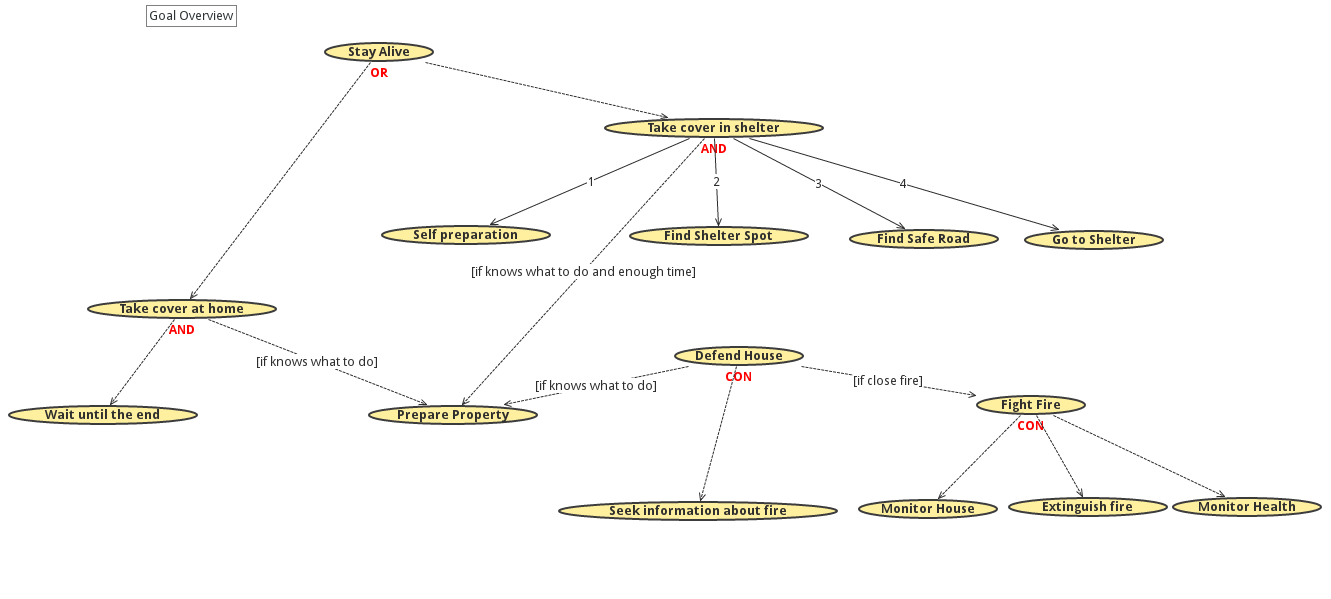
\includegraphics[scale=0.4]{goal-overview.png}
			\caption{\label{fig:goal-overview} Description of the Pedestrian agent goals. Made with the Tactics Development Framework (TDF) plug-in on Eclipse IDE. \cite{tdfwebsite, evertsz2015}}
	  \end{figure}

		The BDI implementation is composed by a main agent called \textquotedblleft Pedestrian\textquotedblright~which corresponds to the Australian citizens.
		Each Pedestrian agent has a health value which decreases according to the injuries caused by the fire and has goals to achieve represented by the figure \ref{fig:goal-overview}.
		At the start, all agent are unaware about the fire and are waiting at home until they perceive a fire.
		At this moment, the agent (represented with a blue circle) chooses its initial intention which can be simply to stay alive or to defend its property.
		This initial objective is determined by the attributes of the agent.
		An agent with a high danger aversion has a bigger chance to leave and take cover.
		However, an agent who is not afraid to fight fire will probably choose to defend his property.

		\subsection{Attributes}

			The Pedestrian agent has two categories of attributes: physical attributes and psychological attributes.
			\newline
			The physical attributes are composed by :
			\begin{itemize}
				\item The health: Corresponds to the health state of the agent. If the health goes down to 0 then the agent dies.
				\item The injuries: Which contains the total amount of damages the fire caused to the agent.
				\item The velocity: Corresponds to the agent speed when it is moving.
			\end{itemize}

			The psychological attributes :
			\begin{itemize}
				\item The determination: Represents the probability to do the action.
				\item The persuadabillity: The probability for the agent to be more or less influenced by others agents or the environment.
				\item The danger aversion: Corresponds to the probability that the agent can accepts the fact that he is in a dangerous situation
				or efraid of the situation.
				\item The perception radius: Determines the perception radius where the agent is able to detect fire.
				\item The danger radius: Correspond to the area where the agent will begin to feel that the situation becomes to be dangerous.
				\item The defense radius: Determines the area where the agent considers that the fire is close enough and must be fought.
			\end{itemize}

		\subsection{Predicates}

			In this implementation we made the choice to simplify the model and to reduce the number of predicates in order to keep a simple model.
			Thus, Pedestrian agents can have only 3 beliefs and 4 desires. The priority of desires can be variable according to the agent attributes. For example,
			an agent a high danger aversion will have a bigger chance to desire to stay alive.

			\paragraph{}
			The agent can believe that :
			\begin{itemize}
				\item it is in a dangerous situation (\textit{belief\_danger}),
				\item it knows a shelter position (\textit{belief\_shelter\_position}),
				\item There are fires (\textit{belief\_fire\_position}).
			\end{itemize}

			The desires :
			\begin{itemize}
				\item \textit{waiting\_for\_event}: The agent can have the desire to wait in order to see how the events will evolve.
				This desire will change according to the danger aversion. Indeed, a person who is afraid will not stay
				and see what happens but will have the desire to \textit{stay alive} instead.
				\item \textit{stay\_alive}: The Pedestrian desires to stay alive (variable according to the danger aversion as well).
				\item \textit{protect\_property}: If it is determined enough to deal with the fire, it can have the desire to protect his property.
				\item \textit{get\_information}: A Pedestrian desires to seek information about the current situation.
			\end{itemize}

		\subsection{Plan}

			\subsubsection{Stay Alive}
				When an agent want to stay alive, he has the possibility to take cover at home or to go in shelters.
				If the agent knows how to fight a fire, he can choose to prepare his property before leaving or before taking cover
				in until the end of the fire. Peoples how want to go in a shelters will make preparation for himself such as take water,
				food or medicines which are represented by the goal \textquotedblleft self preparation\textquotedblright.
				After what, if the agent already knows shelters' position will choose the closest one and determine the safest path
				to use. In contrary, if the agent does not know shelters, it can look around and follow another person who seems to
				know where to go.

			\subsubsection{Defend House}
				An agent who chooses to defend its property will have the choice between three plans.
				The first plan is to look for information using radio, phone or on the web.
				In this simulation we assume the citizens use only the radio.
				If the agent learnt how to fight a fire, the agent has the possibility to prepare its house against the fire.
				Finally if the fire is close to the house, the agent will try to extinguish it.
				According to its knowledge the fire fighting effect will be more or less efficient.
				During the fight, the agent regularly checks the condition of the house and its health condition as well.
				If the agent considers the situation is desperate or if the house burns despite fire fighting, he will
				change its priority and the desire to stay alive will become more important than the desire to defend its property.

			\subsubsection{Death}
				During the simulation an agent may die due to the fire.
				In this implementation, the colour of the agent will switch to black.
				The border colour corresponds to the last agent state before its death.

\chapter{Expectations and Results}

	The experimentation was made 10 times of 500 cycles (time units) with two different sets of parameters for the fire:
	\begin{itemize}
		\item The first experiment was set in order to have a low propagation rate, a moderate probability for
		the fire to grow and ungrow (increase or decrease the fire intensity) but with a low initial intensity:
		\begin{itemize}
			\item Probability of growing: 0.4
			\item Probability of ungrowing: 0.1
			\item Probability of propagation: 0.1
			\item Initial intensity: 1 (max value: 15)
		\end{itemize}
		\item The second experiment was defined as a violent fire, the propagation rate is 3 times more important than
		the first experimentation, the fire has a bigger probability to grow (2 times more) with a bigger initial intensity.
		\begin{itemize}
			\item Probability of growing: 0.8
			\item Probability of ungrowing: 0.1
			\item Probability of propagation: 0.3
			\item Initial intensity: 3 (max value: 15)
		\end{itemize}
	\end{itemize}

	Each simulation begins with exactly 10 fire spots (with a maximum of 50 fires), 200 Citizens, 200 building (one per citizen) and 2 shelters.
	Fires and citizens positions are generated randomly among the remaining free areas, the building positions are exactly the same
	as the citizen positions. That means that all citizens at the initial state are in their house. Only the shelters have
	fixed positions on the bottom left and the top right corner of the map.

	\paragraph{}
	\textbf{Gathered data}
	\paragraph{}

	During each experimentation, we save the last plan used for the agent who died and we categorise each remaining agent which are
	aware of the fire in 5 distinct categories. We have voluntarily reduced the list of the categories described in the chapter \ref{chapter:data}
	from 6 to 5 and decided to merge the category livelihood defenders with the category Can-do defenders. Indeed, the difference between these two
	categories is in the attachment to their home which is not implemented in the currrent simulation.
	\newline
	The results are represented in two differents graphs: The first graph represent the repartition of the last plan used by agents who
	died during the simulation. The second graph contains the profiles of agent who are aware of the fire according to the following
	conditions:
	\begin{itemize}
		\item Unaware reactors: Percentage of agents who used the plan \textit{do\_nothing}, did not try to get cover at home or in a shelter,
		 did not try to seek information, to protect its property and did not try to fight the fire.
		\item Threat avoiders: Percentage of agents who go to shelter instead of staying at home. They do not try to seek information or to fight fire. But they can
		prepare their property before leaving.
		\item Threat monitors: Percentage of agents who take cover at home or go to a shelter and seek information about the fire. They do not try to fight the fire
		but can prepare their property if they want to.
		\item Can-do defenders: Percentage of agents who know what to do during a bushfire (\textit{knows\_how\_to\_fight\_fire}), prepare their property and fight the fire.
		There are no restrictions on the other actions. They can leave, take cover at home or seek information if they wish.
		\item Considered defenders: Percentage of agents who fight fire without knowing how to do it. They do not prepare their property (see the \textit{prepare\_property}
		plan description) but can seek information, get cover at home or leave as well.
	\end{itemize}


	\section{Expected results}

		Among the gathered data, we expect to find in the agent behaviour the profiles described previously in chapter \ref{chapter:data}.
		Moreover, the behaviour should be different according to the fire intensity. An intense fire must produce a bigger psychological
		pressure and increase the number of people who leave earlier. Furthermore, the important fire radiance produced by the fire will
		decrease the number of people who will survive when they choose to take cover at home or when the person tries to fight
		the fire. To finish, an important fire should increase the number of people who will change their mind when they understand that
		the fire is too important to be extinguished. If the fire becomes more intense then the level of agent awareness must increase
		(\textit{Unaware reactors} profil).
		A low fire intensity should show a bigger number of unaware profiles, less people will leave early or will change their mind if they
		are fighting the fire. We can expect as well to see more considered defenders during a low intensity fire than an intense one.


	\section{Current results}

		This section describes the results obtained during the test simulation made. Unfortunatly by lack of time and because
		of issues with GAMA, we did not have time to gather enough data in order to obtain robust results. Thus, this data may be not representative
		of the real agent behaviour because of the randomicity of the different parameters. The very low average of agents dead while they fight fire
		is due to the the randomness of the fire behaviour. The fire can appear near the agent during one cycle and disappear the next cycle. Thus,
		the agent is fighting fire for only one or two cycles and switches back to another plan after that because of the absence of proximity of fire.

		\subsubsection{Low fire intensity}
		\begin{figure}
			\begin{center}
				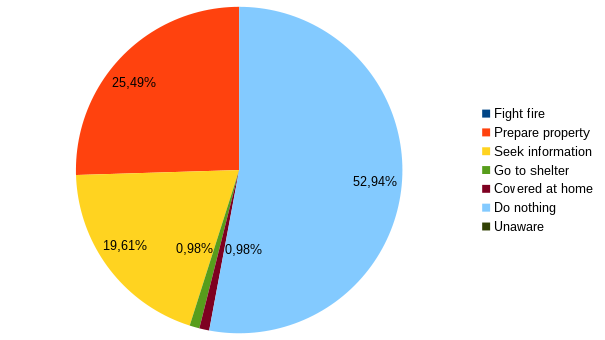
\includegraphics[scale=0.6]{low-lastplan.png}
				\caption{\label{fig:low-lastplan}Low fire \--- last plan used before dying.}
			\end{center}
		\end{figure}

		\begin{figure}
			\begin{center}
				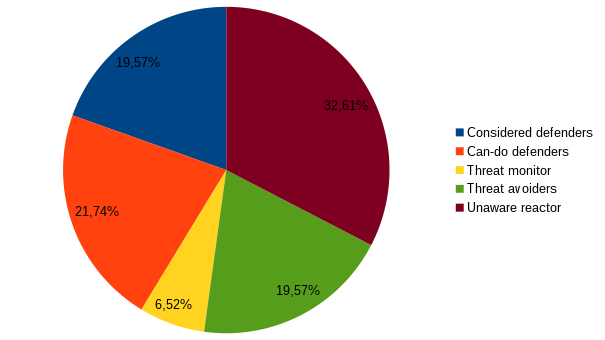
\includegraphics[scale=0.6]{low-profil.png}
				\caption{\label{fig:low-profil}Low fire \--- Agent profile.}
			\end{center}
		\end{figure}

		The figure \ref{fig:low-lastplan} shows that the biggest majority of the Pedestrian agents are dead because of their inactivity
		(\textit{Do nothing} 52.94\%). 25.49\% are dead during the property preparation and 19.61\% during the time where they tried to
		gather information. Very few people are dead during the travel between their house and the shelter and during they were
		covered in their house (both at 0.98\%).
		\newline
		The profile graph (figure \ref{fig:low-profil}) shows that 32.61\% of the agents match with the profile \textit{Unaware reactors}.
		The \textit{Can-do defenders} are the second more represented profile with 21.74\%, followed by the considered defenders and the threat avoiders which are both at 19.57\%.
		Threat monitors are the last profile with 6.52\% of the agents.

		\subsubsection{High fire intensity}

		\begin{figure}
			\begin{center}
				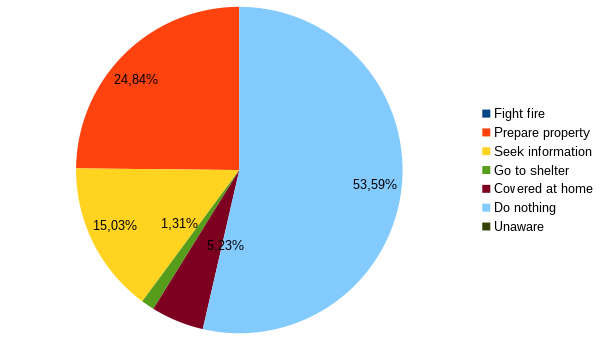
\includegraphics[scale=0.6]{high-lastplan.png}
				\caption{\label{fig:high-lastplan}High fire \--- last plan used before dying (percent values).}
			\end{center}
		\end{figure}

		\begin{figure}
			\begin{center}
				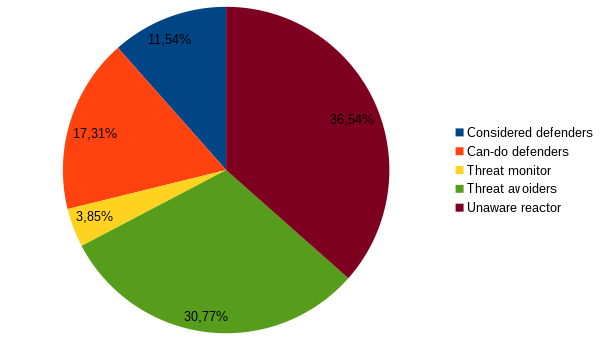
\includegraphics[scale=0.6]{high-profil.png}
				\caption{\label{fig:high-profil}High fire \--- Agent profile (percent values).}
			\end{center}
		\end{figure}

		At first glance, the results seem to be quite similar to the small intensity fire.
		As we can see on the figure \ref{fig:high-lastplan} with an intense fire, more than half of the causes of death are due to an inactivity from the
		Pedestrian agent (53.59\%). The last plan used before dying is the preparation of the property with 24.84\%, and during the research of information (15.03\%).
		5.23\% of dead Pedestrian were sheltered in their house against 1.31\% who died during the travel from the house to the shelter.
		\newline
		The profiles (figure \ref{fig:high-profil}) seem to be similar as well. The first more represented profile is the \textit{Unaware reactor} with 36.54\%.
		followed by the \textit{Threat avoiders} with 30.77\%. The \textit{Can-do defenders} represent 17.31\% against 11.54\% for the \textit{Considered defenders}.
		The \textit{Threat monitors} is again the last profile with 3.85\% of the Pedestrian agents.

		\subsection{Comparison}

		\begin{figure}
			\begin{center}
				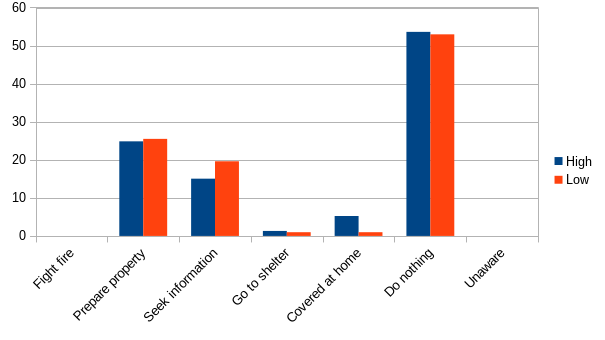
\includegraphics[scale=0.6]{last-plan-comparison.png}
				\caption{\label{fig:last-plan-comparison}Last plan comparison (percent values).}
			\end{center}
		\end{figure}

		\begin{figure}
			\begin{center}
				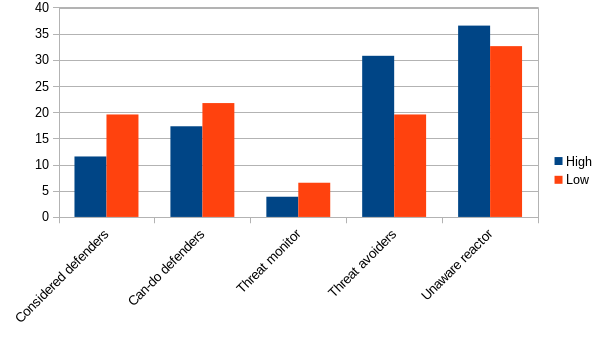
\includegraphics[scale=0.6]{profils-comparison.png}
				\caption{\label{fig:profils-comparison}Profil comparison (percent values).}
			\end{center}
		\end{figure}

		The figure \ref{fig:last-plan-comparison} show that the fire intensity does not influence the cause of death. The two biggest differences can
		be noticed on the percentage of Pedestrians who take cover at home, which is more than 5 times more important during an intense fire than
		during a lower one. This difference can be explained by the fact that an agent who is surrounded by fire will prefer to shelter at home instead of
		crossing the fire in order to go in a shelter. The second notable difference is the percentage of agents who search information during a low fire
		(+4.58\%), which can be explained by the fact that a lower fire includes a lower radiance area than a bigger one. That means an agent in a lower fire will
		have a bigger probability to stay at the plan \textit{seeks\_information} than with an important fire.
		\newline
		The difference between the profiles seems to be more bizarre. Curiously the number of \textit{Unaware reactors} seems to be more
		important during an intense fire than the low intensity fire. However, the difference for the \textit{Threat avoider} profile is more
		realistic in the sense where an intense fire increases the chance to scare an agent. But the current implementation does not take in account the
		fire intensity in the decision making process. This difference is probably due to the low quantity of data gathered with simulations. The last profiles
		correspond better to the expected result, a lower fire increase the number of agents in the profile \textit{Can-do defenders} and \textit{Considered defenders}.
		\paragraph{}
		To conclude, the results shows that the simulation needs to be more detailed on some points and should take more into account
		the fire parameters in order to improve the decision-making process. The distinction between a low intensity fire and an
		important one is too weak (or nonexistant). Moreover, if we make a comparison between the statistics from the VBRC and the BDI
		implementation, we can see that the death causes are not really corresponding. At the exception of the people who were
		passively sheltered in a building (53\% for the simulation against 69\% during the Black Saturday) the results seem not match
		with the reallity. In the futur, we need to define more clarity the related statistics for each profil and death causes.

\chapter{Conclusion}

		In this study we showed that the BDI architecture provides a more intuitive simulation implementation than other simulation
		approaches for human behaviours simulation. However, there are a lack of existing tools for the modelling of BDI agents due
		to the complexity of the language used.
		Consequently, scientists who do not have knowledge in computer science cannot use the tools in their full potential.
		We show an easy way for these scientists to make their own simulation using TDF for the synthesising of textual data such
		as witness statement and GAMA for the simulation making process.
	  The simulation model is still incomplete and can be improved beside some adjustments for a better matching with reality.
		Moreover, the simulation's result does not shows enough similarity with the behaviours described in the witness statements
		despite a too weak distinction between the differents parameters.
  	We tried to have the more simple implementation without lowering descriptiveness in order to find emergent profiles from
		the model. These profils are indeed emerging but do not seem to be correctly proportioned and require more ajustement and
		more implementation improvement.

	\subsubsection{Futur Work}

		In the future, we would like to provide more possibilities to agents.
		Some plans are still incomplete such as \textquotedblleft seek information\textquotedblright ~which
		need an implementation of a radio broadcasting system in order to provide information about fire position to the other agents.
		Many statements show the importance of relationships between agents, such as family, friends, neighbourhood relationships.
		We would like as well to make a comparison between the FSM and the BDI implementation.
		The validation of the simulation will be made by a better comparison with the witness statements and the statistics provided by the CFA.
		\paragraph{}
		The last version of the code is available on github : \url{https://github.com/kust2708/swift.git}.
\backmatter

\bibliographystyle{plain} % plain-fr si rapport en français
\bibliography{bibli}

%En français, il peut être une bonne idée de mettre le résumé en 4e de couverture... (à ce moment là, commenter les abstracts avan la ToC !)
%% 4e de couverture
%\cleardoublepage % Goes to an odd page
%\pagestyle{empty} % no page number
%~\newpage % goes to a new even page
%
%\section*{Abstract} \selectlanguage{english}
%Abstract text
%\medskip
%\selectlanguage{french}
%\section*{Résumé}
%texte de résumé

\end{document}
